\ifx\allfiles\undefined
\documentlecture[12pt, a4paper, oneside, UTF8]{ctexbook}  %  这一句是新增加的
\usepackage[dvipsnames]{xcolor}
\usepackage{amsmath}   % 数学公式
\usepackage{graphicx}
\usetikzlibrary{arrows, calc, decorations.pathmorphing}
\allowdisplaybreaks % 允许公式跨页换行
\newcommand{\pa}{\partial}
\newcommand{\mathminus}{\!\!-\!\!} % 数学环境连字符
\newcommand{\vsup}[1]{\raisebox{-0.1ex}{$\scriptstyle #1$}}
\newcommand{\lsup}[1]{\raisebox{-0.85ex}{$\scriptstyle #1$}}
\definecolor{b1}{RGB}{0,191,255}



\begin{document}
%
 % 单独编译时,其实不用编译封面目录之类的,如需要不注释这句即可
\else
\fi
%  ↓↓↓↓↓↓↓↓↓↓↓↓↓↓↓↓↓↓↓↓↓↓↓↓↓↓↓↓ 正文部分
\part{concise review of basic concepts and definitions}
\chapter{basic concepts , definitions and mathematics}
\section{lecture 1}
\begin{defn}
\par\indent
\begin{enumerate}
    \item \textcolor{b1}{system}:\;
    set of constituents\;(\textbf{not subjected to forces that depend on coordinates of other external constituents})
    \item \textcolor{b1}{property}:\; 
    the system at time \( t \), yields a numerical result \( P(t) \)\;(\textbf{not depend on other instants of time})
    \item \textcolor{b1}{state}:\; 
    the state of the system at time \( t \) is the set of
     (a) the values of the amounts of all constituents,
     (b) the values of the external and internal, and
     (c) the values of all the conceivable properties
\[ A(t) = \{ n_1(t), \cdots, n_r(t), \beta_1(t), \cdots, \beta_s(t), P_1(t), P_2(t), \cdots \} 
\qquad A_1:=A(t_1)\]
\begin{itemize}
    \item \( r\) number of different constituents
    \item \( s\) number of parameters
\end{itemize}
\begin{add}
    Time evolution of the state of the system
    General equation of motion:
\[ \frac{dA(t)}{dt} = f[A(t), \text{forces}(t)] \rightarrow A(t_1)\]

Two theorems of the equation of motion hold for all (well-defined) systems:
\begin{enumerate}
\item First Theorem (Conservation of Linear Momentum)
\item Second Theorem (Conservation of Angular Momentum)
\end{enumerate}
\begin{zhu}
    "well-defined systems"(良好定义的系统)指的是那些能够用明确的数学框架(如拉格朗日力学或哈密顿力学)来描述的系统。
\end{zhu}
\end{add}
    \item \textcolor{b1}{process}:\; 
    specified by
    \begin{itemize}
    \item The initial state of the system
    \item The final state of the system
    \item The effects produced by the interactions with other systems
    \end{itemize}
    \[ A_1 \rightarrow A_2 \]
    \begin{zhu}
        A process simplifies the description of time evolution by abstracting the behavior of a system 
        into a series of state changes over time. 
        
        Instead of detailing \textbf{every instantaneous configuration 
        or interaction}, a process focuses on the overall transformation \textbf{from an initial state to a final state}.
    \end{zhu}
\end{enumerate}
\end{defn}
\begin{defn}
    \par\indent
    \begin{itemize}
        \item Spontaneous Process (no effects on the environment)
        \item Weight Process (external effects are only ``mechanical''(mechanical work))
    \end{itemize}
    \begin{zhu}
    \par\indent
\begin{itemize}
    \item Spontaneous Process 强调了热力学中的不可逆性和能量转换的方向性,将力学中的能量概念与热力学中的熵增联系起来。
    \item Weight Process 将力学中的功与热力学中的能量守恒联系起来。
\end{itemize}
    \end{zhu}
\end{defn}
\begin{law}
    First Law (a unique form):
    \begin{itemize}
    \item \textbf{Assertion 1:} any pair of states \( A_1 \) and \( A_2 \) with 
    compatible values of the amounts of constituents and the parameters of 
    a (well-defined) system \( A \) \textbf{can always be interconnected by} means of a weight process.
    \item \textbf{Assertion 2:} the product \( mg(z_2 - z_1) \) assumes \textbf{the same value for all weight processes} that connect the two given states \( A_1 \) and \( A_2 \).
    \end{itemize}
\end{law}
\begin{corollary}
    Consequences of the First Law:
    \begin{enumerate}
        \item Additivity of energy
        \item Conservation of energy
        \item Exchangeability of energy via interactions
        \item Energy balance equation for a process for system \( A \) (the usual form of the First Law)
    \end{enumerate}
\end{corollary}
\begin{minipage}{0.85\textwidth}
    \centering
    \captionof{table}{Comparison of Steady, Unsteady, Equilibrium, and Nonequilibrium States}
    \begin{tabular}{|p{4cm}<{\centering}|p{4cm}<{\centering}|p{5cm}<{\centering}|}
        \hline
            ~ & ...because of external interactions & ...even if external interactions are turned off \\ 
        \hline
            The state changes with time... & Unsteady state  & Nonequilibrium state \\
        \hline
            The state does not change with time... & Steady state  & Equilibrium state \\ 
        \hline
    \end{tabular}
\end{minipage}
\begin{defn}
    Unstable equilibrium,
    Metastable equilibrium,
Stable equilibrium and

Nonequilibrium
    \par\indent
\begin{minipage}{0.8\textwidth}
    \centering
    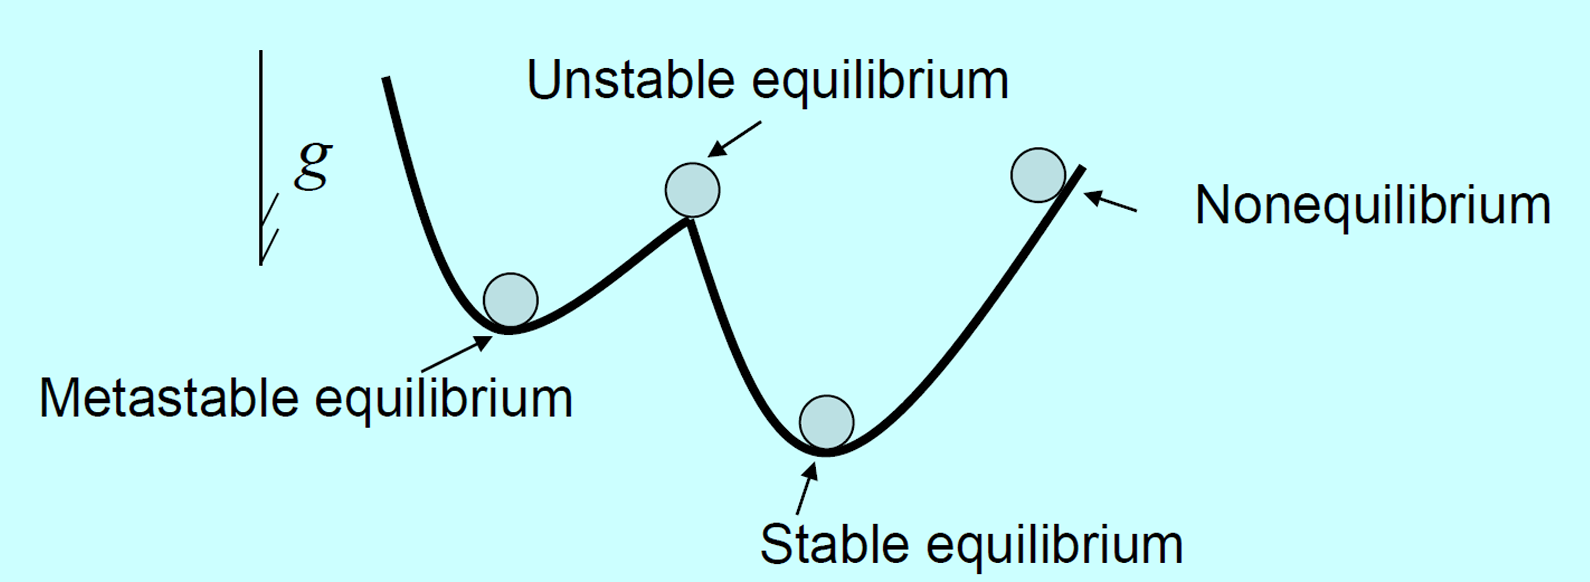
\includegraphics[width=0.75\textwidth]{chap1/image/1.1.png}
\end{minipage}
\end{defn}
\begin{law}
    Second Law:

\begin{itemize}
\item \textbf{Assertion 1:} in the subset of states of a system compatible with 
given values of the amounts of constituents \( n \) and of the parameters \( \beta \), 
there is always \textbf{one and only one SES} for each value of the energy \( E \).  
\item \textbf{Assertion 2:} Starting from any state of the system, it is always possible, 
\textbf{through a reversible weight process}, to reach a SES with arbitrarily fixed, 
\textbf{compatible values of the amounts} of constituents and the parameters.
\end{itemize}
\begin{zhu}
    \par\indent
    \begin{itemize}
    \item \textbf{Mechanics:} One and only one: the stable equilibrium state with minimum energy, \( E_g (n, \beta) \). 
    \item \textbf{Thermodynamics:} One for every value of the energy \( E \)
\end{itemize}
\end{zhu}
\end{law}
\section{lecture 2}
\begin{thm}\label{cfsl1}
    Consequences of First \& Second Law (p\pageref{cfsl2}\;,\; p\pageref{cfsl3})
    \begin{itemize}
        \item Kelvin-Planck statement: impossibility of perpetual motion of the second kind
        
        (It is impossible to extract mechanical energy without other effects from a system initially in a stable equilibrium state)
        \item Clausius statement: Conditions for the spontaneous exchange of energy between systems initially in stable equilibrium states but not in mutual equilibrium
    \end{itemize}
\begin{proof}
    the Kelvin-Planck Statement of the Second Law

\textbf{Ab absurdo:} assume that a PMM2 be possible (further assume, for simplicity of proof here, 
that system \( A \) is composed of two separate parts).

The final states is different from the initial one, and the initial
one was a Steady Equilibrium State.
\end{proof}
\begin{zhu}
    Synonyms of ab absurdo include “reductio ad absurdum,” “proof by contradiction,” and “proof by absurdity.”
\end{zhu}
\end{thm}
\begin{defn}
    The \textbf{adiabatic availability} \( \Psi_1 \) of system \( A \) in state \( A_1 \) 
    measures \textbf{the maximum amount of energy} that \textbf{can be transferred} from the system 
    to a weight in a weight process for \( A \) starting from state \( A_1 \).
    \(\Psi_1=E_1-E_{s1}\)
\end{defn}
\begin{thm}
    Adiabatic availability is a property, but it is \(\underset{\text{lack of utility}}{\text{not additive}}\).
\end{thm}
\begin{defn}
    Mutual stable equilibrium
      
    Two systems \( A \) and \( B \) are in mutual stable equilibrium if their respective states are such that the composite system \( AB \) is in a stable equilibrium state.
\end{defn}
\begin{defn}
    A system \( R \) that in any of its stable equilibrium states is 
    in mutual equilibrium with a given system \( C \) in a given state \( CR \).
    \begin{explain}
        A thermal reservoir, denoted as \(R\), 
        is a system that can exchange energy (typically heat) with another system 
    \(C\) without undergoing any significant change in its own properties.     
    \end{explain}
    \begin{zhu}
        Thermal reservoirs are often used as heat sources or sinks in thermodynamic processes. 
    \end{zhu}
\end{defn}
\begin{proposition}
    It can be proved that the ratio:
\[ \frac{(E_{s2rev}^R - E_{s1}^R)_{A_1 R_{s1} \underset{w,rev}{\rightarrow} A_2 R_{s2rev}}}
{(E_{s2rev}^{R^\circ } - E_{s1}^{R^\circ })_{A_1 R_{s1}^\circ \underset{w,rev}{\rightarrow} A_2 R^\circ _{s2rev} }} 
\]
\begin{itemize}
    \item is positive, 
    \item is independent of \(\begin{cases}
    \text{the initial states}\; R_{s1}, \;R^\circ_{s1}\; \text{of the reservoirs,}\\
    \text{the choice of the auxiliary system} \;A\; \text{and of its states} \; A_1 \;\text{and}\; A_2 , 
    \end{cases}\)
    \item depends solely on the pair of reservoirs \( R \) and \( R^\circ \),
    \item is a dimensionless number.
\end{itemize}
\end{proposition}
\begin{defn}
    property temperature of reservoir \(R\)
\begin{gather*}
T_R=T_{R^\circ}\frac{(E_{s2rev}^R - E_{s1}^R)_{A_1 R_{s1} \underset{w,rev}{\rightarrow} A_2 R_{s2rev}}}
{(E_{s2rev}^{R^\circ } - E_{s1}^{R^\circ })_{A_1 R_{s1}^\circ \underset{w,rev}{\rightarrow} A_2 R^\circ _{s2rev} }} 
\\
\frac{(E_{s2rev}^R - E_{s1}^R)_{A_1 R_{s1} \underset{w,rev}{\rightarrow} A_2 R_{s2rev}}}{T_R}
=\frac{(E_{s2rev}^{R^\circ } - E_{s1}^{R^\circ })_{A_1 R_{s1}^\circ \underset{w,rev}{\rightarrow} A_2 R^\circ _{s2rev}}}{T_{R^\circ}}
\end{gather*}

The ratio 
\begin{itemize}
    \item is independent of reservoir \( R \) and of its initial state \( R_{s1} \)
    \item It depends therefore only on system \( A \) and the pair of states \( A_1 \) and \( A_2 \)
\end{itemize}
\end{defn}
\begin{defn}
    property entropy
    
    The ratio:
\[
\frac{\left(E_{s0\text{rev}}^R - E_{s1}^R\right)_{A_1 R_{s1} \underset{w,rev}{\rightarrow} A_0 R_{s0\text{rev}}}}{T_R}
\]
\begin{itemize}
    \item is independent of reservoir \( R \) and of its initial state \( R_{s1} \)
    \item It depends therefore only on system \( A \) and the pair of states \( A_1 \) and \( A_0 \)
\end{itemize}
\[
S_1 = S_0 + \frac{\left(E_{s0\text{rev}}^R - E_{s1}^R\right)_{A_1 R_{s1} \underset{w,rev}{\rightarrow} A_0 R_{s0\text{rev}}}}{T_R}
\]
\end{defn}
\begin{defn}
    Available Energy w.r.t. a thermal reservoir

    Given state \( A_1 \) and the reservoir \( R \), 
    the maximum weight lift obtains when \( A \) ends 
    in state \( A_R \) and the standard weight process for \( AR \) is reversible.
    \[\Omega_1^R=(E_1-E_R)+(E^R_{s1}-E^R_{sRrev})
    =(E_1-E_R)-(E^R_{sRrev}-E^R_{s1})=(E_1-E_R)-T_R(S_1-S_R)\]
    We call it \textbf{available energy of \(A\) in state \(A_1\) w.r.t. a thermal reservoir \(R\)}.
\end{defn}
\begin{thm}\label{cfsl2}
    Consequences of the (First\&) Second Law (p\pageref{cfsl1}\;,\; p\pageref{cfsl3})
    \begin{itemize}
        \item supports the definition of property adiabatic availability
        \item supports the definition of property temperature of a thermal reservoir
        \item supports the definition of property entropy
        \item The entropy is \textbf{a linear function} of that part of the energy of the system which  
        is unavailable with respect to the reservoir, \textbf{the constant of proportionality} being \textbf{the  
        inverse of the temperature} of the reservoir.
        \begin{center}
            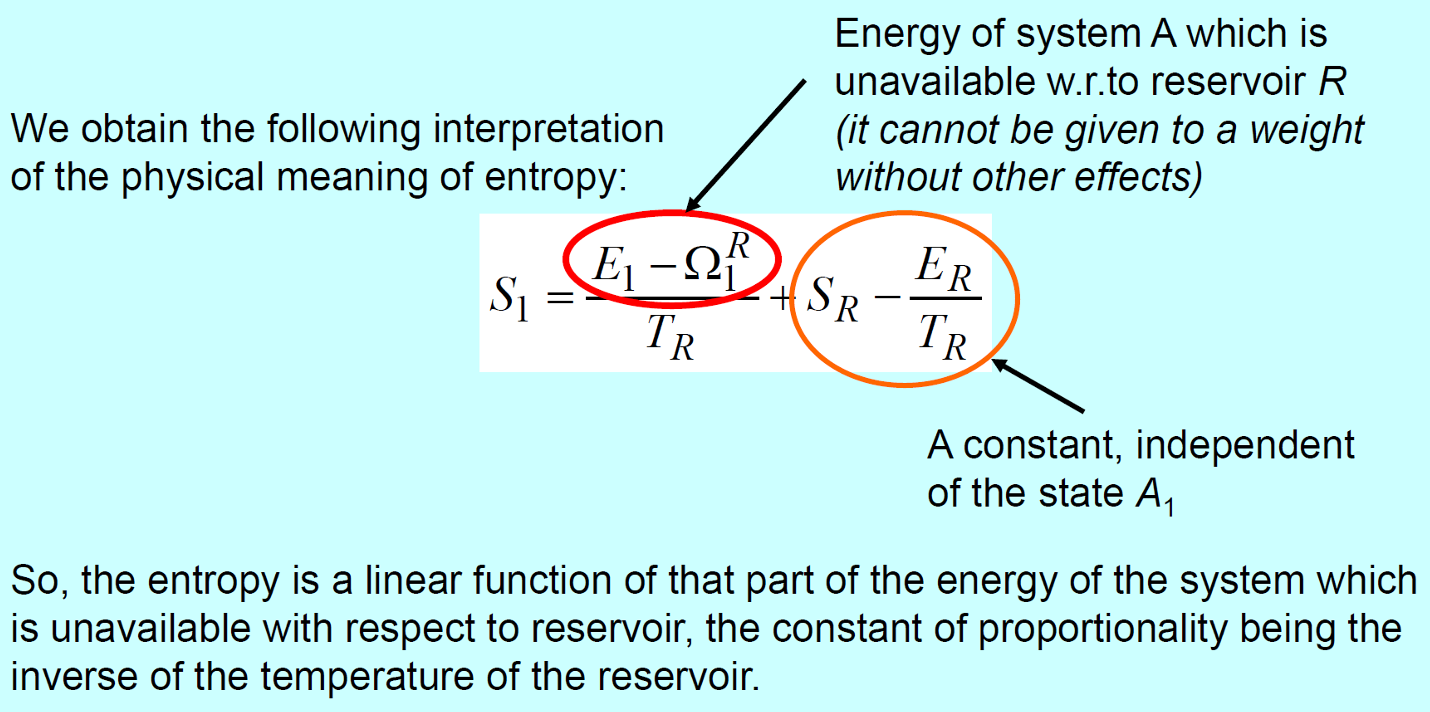
\includegraphics[width=0.7\textwidth]{chap1/image/2.1.png}
        \end{center}
        \item additivity of entropy 
        \item exchangeability of entropy via interactions
        \item principle of entropy non\textminus decrease in a weight process
    \end{itemize}
\end{thm}
\begin{corollary}
    Criteria for the reversibility of a weight process
    \begin{itemize}
        \item \textbf{Reversible iff:} \( E_2 - \Psi_2 = E_1 - \Psi_1 \qquad
        E_2 - \Omega^R_2 = E_1 - \Omega^R_1 \qquad S_2=S_1\)
        \item \textbf{Irreversible iff:} \( E_2 - \Psi_2 \geq E_1 - \Psi_1 \qquad
        E_2 - \Omega^R_2 \geq E_1 - \Omega^R_1 \qquad S_2\geq S_1 \)
        \item \textbf{Impossible iff:} \( E_2 - \Psi_2 \leq E_1 - \Psi_1 \qquad
        E_2 - \Omega^R_2 \leq E_1 - \Omega^R_1 \qquad S_2\leq S_1 \)
    \end{itemize}
\end{corollary}
\begin{principle}

\textbf{Maximum entropy principle:} Among all the states with the same given values of the amounts of constituents, the parameters, and \textbf{the energy}, only the stable equilibrium state has the maximum value of the entropy.

\textbf{Minimum energy principle:} Among all the states with the same given values of the amounts of constituents, the parameters, and \textbf{the entropy}, only the stable equilibrium state has the minimum value of the energy.
\begin{add}
    \textbf{非平衡态系统中最小能量原理失效}:
        \begin{itemize}
            \item 传统热力学中,系统趋向能量最低态的前提是孤立或平衡条件。
            \item 非平衡态系统的能量可能被外部驱动力“泵入”,导致能量高于平衡态(如生物细胞的主动运输)。
        \end{itemize}
\end{add}
\end{principle}
\begin{thm}\label{cfsl3}
    Consequences of the (First\&) Second Law (p\pageref{cfsl1}\;,\; p\pageref{cfsl2})
\begin{itemize}
    \item State Principle
    
    Among all the states with the same given values of the amounts of constituents, the parameters, 
    and the energy, one and only one is a stable equilibrium state (Second Law) and 
    therefore the value of any property is uniquely determined by the values of 
    the amounts of constituents, the parameters, and the energy.
    \[
    P = P(E, n_1, \ldots, n_r, \beta_1, \ldots, \beta_s)
    \] 
    \item Gibbs relation
    \begin{itemize}
        \item 
        \(
        S = S(E, V, n_1, \dots, n_r)
        \),        
        Gibbs relation (entropy form):
\[
dS = \frac{1}{T} dU + \frac{P}{T} dV - \sum_i \frac{\mu_i}{T} dn_i
\]
        \item 
        \(
        E = E(S, V, n_1, \dots, n_r)
        \),        
        Gibbs relation (energy form):
        \[
        dE = T dS - P dV + \sum_i \mu_i dn_i
        \]
    \end{itemize}
    \begin{add}
        通过诺特定律,Gibbs 关系的能量形式和熵形式可以统一解释为:
\begin{itemize}
    \item 能量形式:时间平移对称性生成的守恒内能 \(E\),描述了系统的守恒性质。
    \item 熵形式:熵最大化原理,描述了系统在自发过程中熵的变化方向。
\end{itemize}
        两种形式通过 Legendre 变换和对偶对称性紧密关联。
    \begin{zhu}
        热力学中常见的对称性:

    时间平移对称性 $\Rightarrow$ 能量守恒,
    空间均匀性 $\Rightarrow$ 压强平衡,
    粒子数守恒 $\Rightarrow$ 化学势平衡。
    \end{zhu}
    \end{add}
\end{itemize}
\end{thm}
\begin{defn}
    \par\indent
    \begin{itemize}
        \item The (absolute) temperature is defined by  
        \[
        T = \left( \frac{\partial E}{\partial S} \right)_{\vec{n}, V} \quad \text{or} \quad \left( \frac{\partial S}{\partial E} \right)_{\vec{n}, V} = \frac{1}{T}
        \]          
        \item The chemical potential of the \(i\)-th constituent is defined by  
        \[
        \mu_i = \left( \frac{\partial E}{\partial n_i} \right)_{S, V} \quad \text{or} \quad \left( \frac{\partial S}{\partial n_i} \right)_{E, V} = -\frac{\mu_i}{T}
        \]          
        \item The pressure is defined by  
        \[
        p = - \left( \frac{\partial E}{\partial V} \right)_{S, \vec{n}} \quad \text{or} \quad \left( \frac{\partial S}{\partial V} \right)_{E, \vec{n}} = \frac{p}{T}
        \]
    \end{itemize}
\end{defn}
\section{lecture 3}
\begin{proposition}
    Necessary Conditions for Mutual Equilibrium
    \begin{itemize}
        \item \((T_1=T_2)\)
        \textbf{Equality of the temperatures} of the two systems is a necessary condition for mutual equilibrium if the two systems can exchange \textbf{energy}.
        \item \((p_1=p_2)\)
        \textbf{Equality of the pressures} of the two systems is a necessary condition for mutual equilibrium if the two systems can exchange \textbf{volume}.
        \item \((\mu_{i,1} = \mu_{i,2})\)
        \textbf{Equality of the chemical potentials of the \(i\)-th constituent} in the two systems is a necessary condition for mutual equilibrium if the two systems can exchange \textbf{the \(i\)-th constituent}.
    \end{itemize}
\end{proposition}
\begin{minipage}{0.8\textwidth}
    \centering
    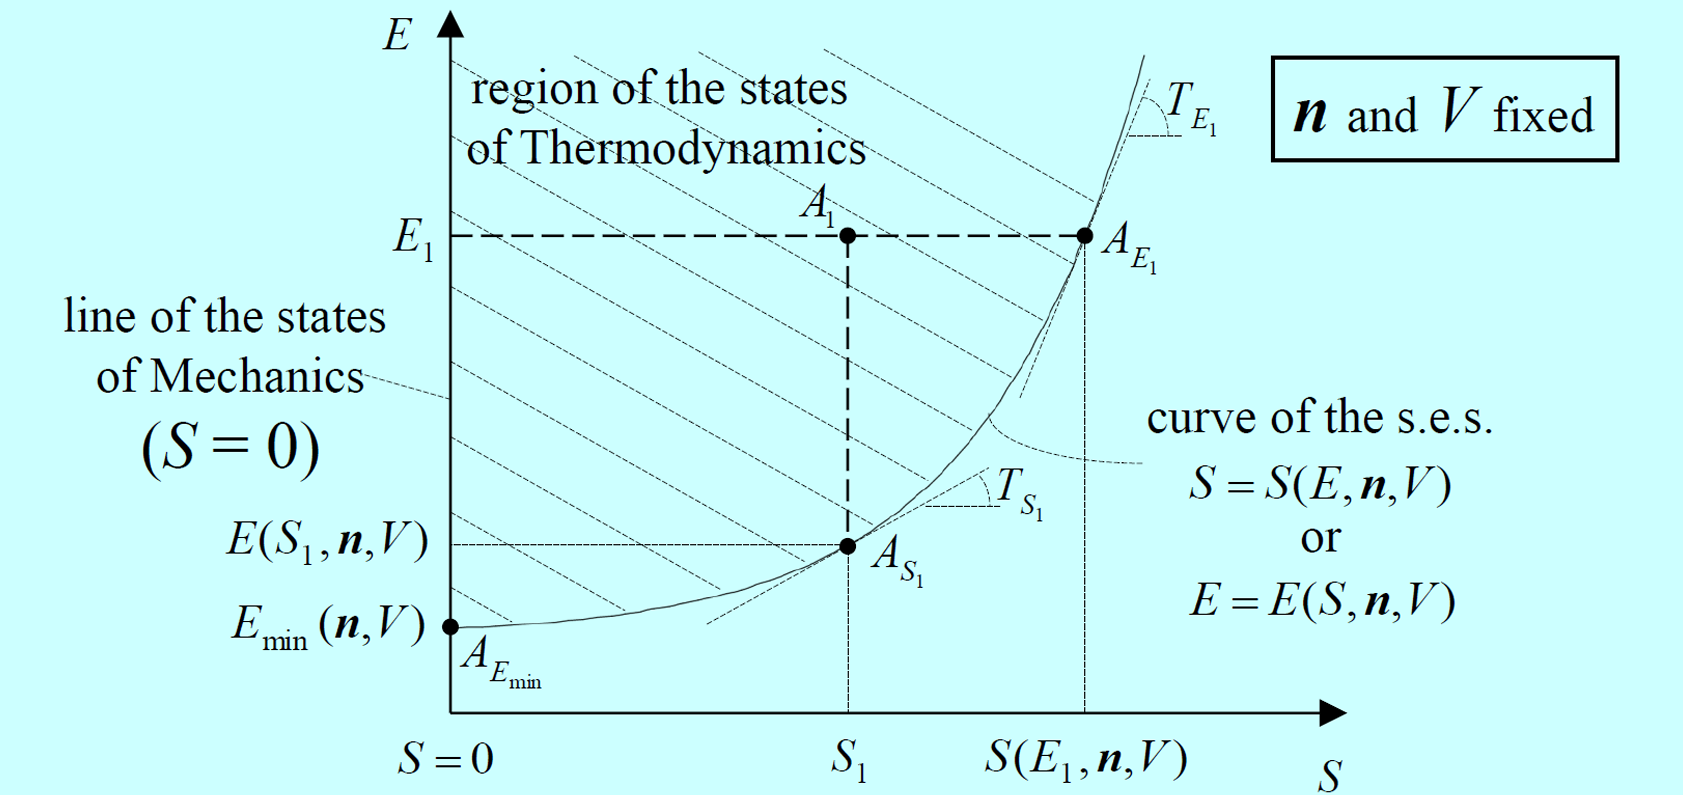
\includegraphics[width=0.75\textwidth]{chap1/image/3.1.png}
    \captionof{figure}{Representation of notSES and SES}
\end{minipage}
\begin{defn}
    negative temperatures \(T_{N1}\)

\begin{minipage}{0.8\textwidth}
    \centering
    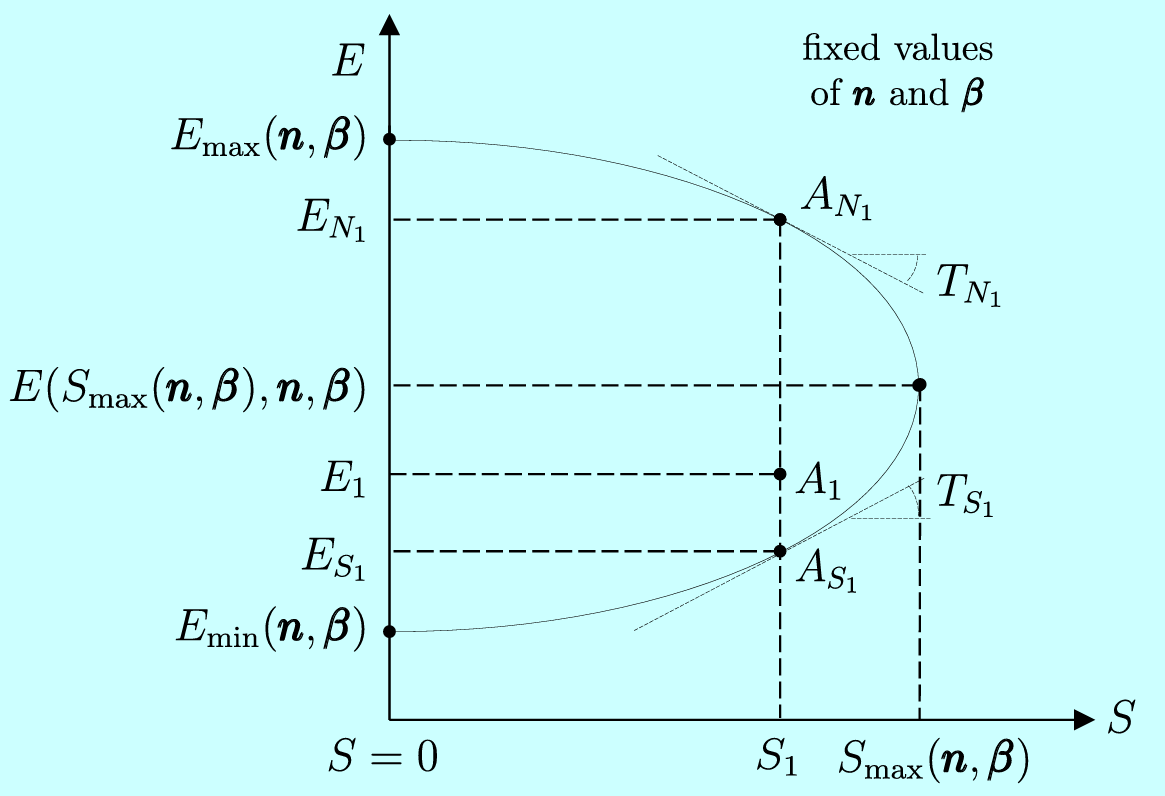
\includegraphics[width=0.5\textwidth]{chap1/image/3.2.png}
    \captionof{figure}{Special systems with upper bounded energy}
\end{minipage}
\end{defn}
\section{lecture 4}
\begin{thm}
    \indent
    \begin{itemize}
        \item To extract energy from a system in a s.e.s., we must also extract entropy:
        \[
        S_{s1} - S_{s2} > (E_{s1} - E_{s2}) / T_{s1}
        \]
        \item To give entropy to a system in a s.e.s., we must also give energy:
        \[
        E_{s2} - E_{s1} > T_{s1}(S_{s2} - S_{s1})
        \]
    \end{itemize}
    \begin{add}
\begin{itemize}
    \item \textbf{能量与熵的不可分割性}  
    \[
    S_{s1} - S_{s2} > \frac{E_{s1} - E_{s2}}{T_{s1}}
    \]
    \textit{哲学内涵}:能量(阳)显化为外在功用时,系统内禀的微观状态自由度(阴)必须同步减少,以熵的隐性耗散为代价。
    \[
    E_{s2} - E_{s1} > T_{s1}(S_{s2} - S_{s1})
    \]
    \textit{哲学内涵}:熵增(阴)代表系统微观状态自由度的扩展,而能量输入(阳)则是维持这种扩展的必要动力。
    \item \textbf{动态平衡}  
    
    系统稳态(s.e.s.)下的状态迁移需满足:
    \[
    \Delta E > T\Delta S \quad \text{或} \quad \Delta S > \frac{\Delta E}{T}
    \]
    \textit{哲学内涵}:阴阳消长需通过能量\textminus 熵交换(冲气)达成新平衡。不等式方向表明:
    \begin{itemize}
        \item 当系统释放能量(阳减),必伴随熵的净输出(阴减),否则平衡被破坏
        \item 当系统吸收熵(阴增),需注入超额能量(阳增)以维持(和)的状态
    \end{itemize}

    \item \textbf{自然无为的约束 (为者败之,执者失之) }
    
    由于The Onsager reciprocity relations,对传热、扩散等过程,熵产率(\(\sigma\))与热力学力(\(X\))和流(\(J\))满足:
    \[
    \sigma = J \cdot X \geq 0
    \]
在近平衡态下,流与力呈线性关系 \(J = L X\),故:
\[
\dot{S}_{\text{gen}} = \int_V \sigma \, dV \geq 0 \quad \text{且} \quad \sigma \propto X^2 \; (\text{近平衡态})
\]
干预系统时,损耗能量满足:
\[
\dot{W}_{\text{lost}} = T_R \dot{S}_{\text{gen}} \propto X^2 
\]
\textbf{典型耗散形式}:
\begin{itemize}
\item \textbf{焦耳加热:}电阻为 \(R\) 时,功率损耗 \(P = I^2 R\),与电流平方成正比。
\item \textbf{粘滞耗散:} 流体剪切速率为 \(\dot{\gamma}\) 时,耗散率 \( \Psi = \eta \dot{\gamma}^2 \),其中 \(\eta\) 为粘度。
\item \textbf{温差传热:} 温度梯度为 \(\nabla(T)\) 时,熵产率为 \( \sigma = \kappa \frac{(\nabla T)^2}{T^2} \),其中 \(\kappa\) 为热导率。
\end{itemize}
    对系统的能量\textminus 熵操控必然引入不可逆代价,卡诺循环效率仅为理论极限。
\end{itemize}
    \end{add}
\end{thm}
\begin{thm}
    Necessary conditions for mutual equilibrium

    \begin{zhu}
        Classification of Concavity
        \par\indent
        \textbf{Concave}: Concave (mathematical concavity, represented by $\leq$ 0 for second derivatives)
        \par\indent
        \textbf{Convex}: Convex (mathematical convexity, represented by $\geq$ 0 for second derivatives)        
    \end{zhu}
    If \( A \) and \( B \) are in Mutual Stable Equilibrium in states \( A_0 \) and \( B_0 \), then \( C_0 \) is a SES. 
    Then, the Maximum Entropy Principle implies that \( C_1 \) cannot be a SES and therefore \( S^C_1 < S^C_0 \), 
    i.e. the strict inequality:
    \(S^C_1 - S^C_0 < 0\)
    \begin{enumerate}
        \item \textbf{Temperature and Pressure} Equality at Mutual Equilibrium
        \begin{itemize}
            \item From entropy additivity:
        \begin{align*}
                S^C_1 - S^C_0 &= (S^A_1 + S^B_1) - (S^A_0 + S^B_0) = (S^A_1 - S^A_0) + (S^B_1 - S^B_0)\\
                &\approx \frac{1}{T^A_0} dE + \frac{p^A_0}{T^A_0} dV + \frac{1}{2} d^2_{E,V} S^A 
                + \frac{1}{T^B_0} (-dE) + \frac{p^B_0}{T^B_0} (-dV) + \frac{1}{2} d^2_{E,V} S^B \\
                &= \underbrace{\left( \frac{1}{T^A_0} - \frac{1}{T^B_0} \right)}_{=0} dE 
                + \underbrace{\left( \frac{p^A_0}{T^A_0} - \frac{p^B_0}{T^B_0} \right)}_{=0} dV 
                + \frac{1}{2} d^2_{E,V} S^A + \frac{1}{2} d^2_{E,V} S^B < 0
        \end{align*}
        \item For the inequality to hold for all choices of \( dE \) and \( dV \), 
        the terms in brackets must be zero. Therefore, the second-order differentials must be negative, 
        i.e. the fundamental relation is \textbf{concave} in \( E \) and \( V \):
\begin{align*}
            d_{E,V}^2 S &= \frac{\partial^2 S}{\partial E^2} (dE)^2 + 2 \frac{\partial^2 S}{\partial E \partial V} dEdV + \frac{\partial^2 S}{\partial V^2} (dV)^2 < 0
            \\&\Rightarrow
            \begin{cases} 
            \frac{\partial^2 S}{\partial E^2} < 0 \qquad \frac{\partial^2 S}{\partial V^2} < 0 \\ 
            \frac{\partial^2 S}{\partial E^2} \frac{\partial^2 S}{\partial V^2} - \left[ \frac{\partial^2 S}{\partial E \partial V} \right]^2 < 0 
            \end{cases}
\end{align*}
\begin{zhu}\label{<>}
    这里Beretta教授在幻灯片上写的是
    \[
        d_{E,V}^2 S = \frac{\partial^2 S}{\partial E^2} (dE)^2 + 2 \frac{\partial^2 S}{\partial E \partial V} dEdV + \frac{\partial^2 S}{\partial V^2} (dV)^2 \boxed{\leq} 0
    \]
    这是一般化的。方程中的“$\leq0$”在大多数情况下都取“$<0$”,使得Hessian矩阵负定,确保所有方向扰动均使熵减少。
    为了强调大多数情况只能取严格不等号,我对此进行了修改。

    在热力学稳定性分析中,当两个系统 \( A \) 和 \( B \) 处于平衡时,总熵的二阶变化必须严格小于零(\(<0\))以确保平衡的稳定性。
    推导中第一个方程的总变化严格小于零是合理的,因为一阶项为零(平衡条件)后,二阶项之和必须负定(严格凹)。
    然而,第二个方程中熵的二阶微分 \( d^2_{E,V} S \leq 0 \) 是熵作为一般凹函数的性质,允许半负定(如相变临界点)。
    但在稳定性条件下,系统熵的二阶微分应严格负定(\(<0\)),若仅 \( \leq 0 \),可能存在非零扰动使总变化为零,破坏稳定性。
    
    在“\textbf{Temperature and Potential} Equality at Mutual Equilibrium”部分中,同样出于类似的原因,我已对其进行修改,因此不再在相关位置逐一说明。
\end{zhu}
        \end{itemize}
        \item \textbf{Temperature and Potential} Equality at Mutual Equilibrium
        \begin{itemize}
            \item From entropy additivity:
            \begin{align*}
                S^C_1 - S^C_0 &= (S^A_1 + S^B_1) - (S^A_0 + S^B_0) = (S^A_1 - S^A_0) + (S^B_1 - S^B_0)\\
                &\approx \frac{1}{T^A_0} dE - \frac{\mu^A_{i0}}{T^A_0} dn_i + \frac{1}{2} d^2_{E,n_i} S^A
                + \frac{1}{T^B_0} (-dE) - \frac{\mu^B_{i0}}{T^B_0} (-dn_i) + \frac{1}{2} d^2_{E,n_i} S^B\\
                &= \underbrace{\left( \frac{1}{T^A_0} - \frac{1}{T^B_0} \right)}_{=0} dE + \underbrace{\left( \frac{\mu^B_{i0}}{T^B_0} 
                - \frac{\mu^A_{i0}}{T^A_0} \right)}_{=0} dn_i + \frac{1}{2} d^2_{E,n_i} S^A + \frac{1}{2} d^2_{E,n_i} S^B < 0
            \end{align*}
                \item For the inequality to hold for all choices of \( dE \) and \( dn_i \), 
                the terms in brackets must be zero. Therefore, the second-order differentials must be negative, 
                i.e. the fundamental relation is \textbf{concave} in \( E \) and \( n_i \):          
\begin{align*}
                d^2_{E,n_i} S &= \frac{\partial^2 S}{\partial E^2} (dE)^2 + 2 \frac{\partial^2 S}{\partial E \partial n_i} dEdn_i + \frac{\partial^2 S}{\partial n_i^2} (dn_i)^2 < 0\\
                &\Rightarrow
                \begin{cases} 
                \frac{\partial^2 S}{\partial E^2} < 0 \qquad \frac{\partial^2 S}{\partial n_i^2} < 0 \\ 
                \frac{\partial^2 S}{\partial E^2} \frac{\partial^2 S}{\partial n_i^2} - \left[ \frac{\partial^2 S}{\partial E \partial n_i} \right]^2 < 0 
                \end{cases}
\end{align*}
        \end{itemize}
    \item Concavity of the fundamental relation (introducing the Hessian matrix)

    The fundamental relation is \textbf{concave} in all its independent variables, 
    i.e. in any SES the Hessian of the fundamental relation \( S = S(E, n, V) \) 
    is a negative semidefinite matrix:
    \[
    \text{Hessian}(S) =
    \begin{bmatrix}
    \frac{\partial^2 S}{\partial E^2} & \frac{\partial^2 S}{\partial E \partial n_1} & \cdots & \frac{\partial^2 S}{\partial E \partial n_r} & \frac{\partial^2 S}{\partial E \partial V} \\
    \frac{\partial^2 S}{\partial n_1 \partial E} & \frac{\partial^2 S}{\partial n_1^2} & \cdots & \frac{\partial^2 S}{\partial n_1 \partial n_r} & \frac{\partial^2 S}{\partial n_1 \partial V} \\
    \vdots & \vdots & \ddots & \vdots & \vdots \\
    \frac{\partial^2 S}{\partial n_r \partial E} & \frac{\partial^2 S}{\partial n_r \partial n_1} & \cdots & \frac{\partial^2 S}{\partial n_r^2} & \frac{\partial^2 S}{\partial n_r \partial V} \\
    \frac{\partial^2 S}{\partial V \partial E} & \frac{\partial^2 S}{\partial V \partial n_1} & \cdots & \frac{\partial^2 S}{\partial V \partial n_r} & \frac{\partial^2 S}{\partial V^2}
    \end{bmatrix}
    \]
    \[
    d^2 S_{E,n,V} = (dE, dn_1, \ldots, dn_r, dV) \cdot \text{Hessian}(S) \cdot (dE, dn_1, \ldots, dn_r, dV)^T \leq 0
    \]
\end{enumerate}
    \begin{add}
    基本关系 $S = S(E, n, V)$ 的凹性推论
\begin{enumerate}
  \item \textbf{熵极大值原理}:平衡态熵 $S$ 达极大值,Hessian 负半定保证全局极大,即
        \[
          d^2 S \leq 0 \quad \forall \, (dE, dn_1, \dots, dn_r, dV) \neq \vec{0}
        \]
  \item \textbf{热力学稳定性条件}:
        \[
          \frac{\partial^2 S}{\partial E^2} \leq 0 \Rightarrow C_V \geq 0 \qquad
          \frac{\partial^2 S}{\partial n_i^2} \leq 0 \Rightarrow \left(\frac{\partial \mu_i}{\partial n_i}\right)_{\!T,V} \leq 0 \qquad
          \frac{\partial^2 S}{\partial V^2} \leq 0 \Rightarrow \kappa_T \geq 0
        \]
  \item \textbf{Le Chatelier 原理}:
    从熵的凹性 \( S = S(E, V, n) \) 出发,Hessian 矩阵负半定:
    \[
    d^2 S = \sum_{i,j} \frac{\partial^2 S}{\partial x_i \partial x_j} dx_i dx_j \leq 0 \quad (x = (E, \vec{n}, V))
    \]
    对扰动 \( dE \) 和响应 \( dT \):
    \[
    \frac{\partial}{\partial E} \left( \frac{1}{T} \right) = -\frac{1}{T^2} \frac{\partial T}{\partial E} 
    = \frac{\partial^2 S}{\partial E^2} \leq 0 \quad \Rightarrow \quad \frac{\partial T}{\partial E} \geq 0
    \]
    系统响应削弱扰动,如
        \[
          dV < 0 \Rightarrow dP > 0 \qquad dE > 0 \Rightarrow dT > 0
        \]
  \item \textbf{热力学势凸性}:通过 Legendre 变换,熵的凹性可以转化为其他热力学势的凸性
        \[
          U(S,V,n)\text{ 凸}\qquad F(T,V,n)\text{ 凹}\qquad G(T,P,n)\text{ 凹}
        \]
  \item \textbf{热力学极限存在性}:熵凹性保证宏观极限下热力学量(如 $S$, $U$)存在且唯一。
\end{enumerate}
    \end{add}
\end{thm}
\begin{example}
    Surface tension and Young-Laplace equation

    If \( B, C, D \) are in MSE in states \( B_0, C_0, D_0 \), then \( F_0 \) is a SES. 
    Then, the MEP implies that \( F_1 \) cannot be a SES and therefore \( S^F_1 < S^F_0 \), 
    i.e. the strict inequality:
    \(
    S^F_1 - S^F_0 < 0
    \)
\begin{itemize}
    \item From entropy additivity:
    \begin{gather*}
        \text{Assuming}\quad T_0^B = T_0^C = T_0^D = T_0 \qquad dE^B + dE^C + dE^D = 0 \\
        \mu_{i0}^B = \mu_{i0}^C = \mu_{i0}^D = \mu_{i0} \qquad 
        dm_i^B + dm_i^C + dm_i^D = 0 \;,\; \forall i \qquad
        dV^B = -dV^D
    \end{gather*}
\begin{align*}
        S^F_1 - S^F_0 &= (S^B_1 + S^C_1 + S^D_1) - (S^B_0 + S^C_0 + S^D_0) \\
        &= (S^B_1 - S^B_0) + (S^C_1 - S^C_0) + (S^D_1 - S^D_0)\\
        &= \frac{1}{T^B_0} dE^B + \frac{p^B_0}{T^B_0} dV^B 
        + \frac{1}{T^C_0} dE^C - \frac{\sigma^C_0}{T^C_0} dA^C 
        + \frac{1}{T^D_0} dE^D + \frac{p^D_0}{T^D_0} dV^D +\cdots \\
        &= \frac{1}{T_0} \left[ (p^D_0 - p^B_0) dV^D - \sigma^C_0 dA^C \right] + \cdots < 0
\end{align*}
    \item Assuming \( C \) has spherical shape of radius \( R \):
    \[
    p^D_0 - p^B_0 = \frac{2\sigma^C_0}{R}
    \]
    \item Assuming \( C \) has cylindrical shape of radius \( R \) and length \( L \):
    \[
    p^D_0 - p^B_0 = \frac{\sigma^C_0}{R}
    \]
    \item Assuming small local displacement \( de = de|_{\theta_1,\theta_2} \),
\begin{gather*}
        A^C = \iint_C R_1R_2 \, d\theta_1 \, d\theta_2 \quad dV^D 
        = \iint_C R_1R_2 \, de \, d\theta_1 \, d\theta_2\\
        dA^C = \iint_C [(R_1 + de)(R_2 \pm de) - R_1R_2] \, d\theta_1 \, d\theta_2 
        \approx \iint_C (\pm R_1 + R_2) \, de \, d\theta_1 \, d\theta_2\\
        \Downarrow\\
        \iint_C [(\rho_0^D - p_0^B) \, R_1R_2 - \sigma_0^C (\pm R_1 + R_2)]_{\theta_1,\theta_2} \, de 
        \, d\theta_1 \, d\theta_2 = 0 \quad \forall de\\
        \Downarrow\\
\left[ \frac{1}{R_1} \pm \frac{1}{R_2} \right]_{\theta_1, \theta_2} = \frac{p_0^D - p_0^B}{\sigma_0^C}
\\ \Downarrow\\
        p_0^D - p_0^B = 
        \sigma_0^C \left[ \frac{1}{R_1} \pm \frac{1}{R_2} \right]_{\theta_1, \theta_2}
\end{gather*}
\end{itemize}
\end{example}
\begin{thm}
    Clausius inequality
\begin{itemize}
    \item infinitesimal transfers
\[
\frac{\delta E^{A \rightarrow B}}{T_1^A} \leq \delta S^{A \rightarrow B} - \delta S_{\text{irr}}^A \leq \delta S^{A \rightarrow B} \leq \delta S^{A \rightarrow B} + \delta S_{\text{irr}}^B \leq \frac{\delta E^{A \rightarrow B}}{T_1^B}
\;\text{irr:=irreversible process}
\]
\begin{center}
    \includegraphics*[width=0.6\textwidth]{chap1/image/3.3.png}
\end{center}
    \item finite transfers
    
    Systems \( A \) and \( B \) are initially in SES and interact directly without other effects by 
    exchanging a finite amount \( E^{A \to B} \) of energy. Such exchange can occur only if 
    there is also an entropy \( S^{A \to B} \) transfer, at least \( S^{A \to B} |_{\min} \) but 
    no more than \( S^{A \to B} |_{\max} \).
    \[
    S_{\text{SES}}^B (E_1^B + E_2^{A \to B}, V^B, n^B) - S_1^B \leq S_2^{A \to B} 
    \leq S_1^A - S_{\text{SES}}^A (E_1^A - E_2^{A \to B}, V^A, n^A)
    \]
    \begin{center}
        \includegraphics*[width=0.6\textwidth]{chap1/image/3.4.png}
    \end{center}
\end{itemize}
\end{thm}
\section{lecture 5}
\begin{defn}
    Types of interactions

    \begin{itemize}
        \item \textbf{Work interaction}: when energy is exchanged with no exchange of 
        \textbf{entropy} nor amounts of \textbf{constituents}. 
        \item \textbf{Adiabatic process}: a process whereby the system experiences \textbf{only work interactions}.
        \item \textbf{Non-work interaction}: there is an exchange of \textbf{entropy} or \textbf{constituents}. 
        \item \textbf{Non-adiabatic process}: there are some \textbf{non-work interactions}.
        \item \textbf{Heat interaction}: a limiting case of \textbf{a non-work interaction with no exchange of constituents} 
        in which the energy exchanged is entirely distinguishable from work. It occurs between two systems initially in 
        stable equilibrium states with an exchange of both energy and entropy between the two systems, 
        such that the exchanged energy is called heat.

        The max fraction of the exchanged energy that can be separated as \textbf{work is negligible} (\(< 1\)) only 
        in the limit \( T_1^A \rightarrow T_1^B \) that is if:
    \(
    \frac{T_1^A - T_1^B}{T_1^A} \ll 1
    \).
    \end{itemize}
\end{defn}
\begin{example}
    First and second law 
    efficiency
     in
     heat engines,
     heat pumps and
    refrigeration
\end{example}
\begin{defn}
    Definitions of other SES properties and their respective relations 
    in terms of \( p, V, T, C_v, C_p, \gamma = \frac{C_p}{C_v}, \kappa_T, \alpha_P \).
\begin{itemize}
\item 
\textbf{The Mayer relation} is defined as the difference 
between the heat capacities at constant pressure and constant volume.
\begin{align*}
C_p - C_v &=\left( \frac{\partial H}{\partial T} \right)_{p, \vec{n}}
-\left( \frac{\partial E}{\partial T} \right)_{V, \vec{n}}\\
&= \left( \frac{\partial E}{\partial T} \right)_{p, \vec{n}} 
+ \left( \frac{\partial (pV)}{\partial T} \right)_{p, \vec{n}} 
- \left( \frac{\partial E}{\partial T} \right)_{V, \vec{n}} \\
&= \left( \frac{\partial E}{\partial T} \right)_{p, \vec{n}} 
+ p \left( \frac{\partial V}{\partial T} \right)_{p, \vec{n}} 
- \left( \frac{\partial E}{\partial T} \right)_{V, \vec{n}} \\
&= \left( \frac{\partial E}{\partial T} \right)_{V, \vec{n}} + 
\left( \frac{\partial E}{\partial V} \right)_{T, \vec{n}} 
\left( \frac{\partial V}{\partial T} \right)_{p, \vec{n}} 
-\left( \frac{\partial E}{\partial T} \right)_{V, \vec{n}}
+ p \left( \frac{\partial V}{\partial T} \right)_{p, \vec{n}} \\
&= \left(\left( \frac{\partial E}{\partial V} \right)_{T, \vec{n}} 
+ p \right)\left( \frac{\partial V}{\partial T} \right)_{p, \vec{n}} 
= \left( -p + T \left( \frac{\partial p}{\partial T} \right)_V \right) \left( \frac{\partial V}{\partial T} \right)_{p, \vec{n}} 
+ p \left( \frac{\partial V}{\partial T} \right)_{p, \vec{n}} \\
&= \boxed{T \left( \frac{\partial V}{\partial T} \right)_p 
\left( \frac{\partial p}{\partial T} \right)_V }
=\boxed{- T \left( \frac{\partial V}{\partial T} \right)_p 
\frac{\left( \frac{\partial V}{\partial T} \right)_p}
{\left( \frac{\partial V}{\partial p} \right)_T}} 
=\boxed{\frac{TV \alpha_p^2}{\kappa_T}}
\end{align*}
\item 
\textbf{The Joule-Thomson coefficient} \(\mu_{JT}\) is given by:
\begin{align*}
    \mu_{JT} &= \left( \frac{\partial T}{\partial p} \right)_H \\
&\boxed{\begin{gathered}
    \because \; dH = T \left( \frac{C_p}{T} dT - 
    \left( \frac{\partial V}{\partial T} \right)_p dp \right) + V dp=0
    \\\therefore\; 
    C_p dT = \left( T \left( \frac{\partial V}{\partial T} \right)_p - V \right) dp
\end{gathered}}
    \\&= \frac{1}{C_p} \left( T \left( \frac{\partial V}{\partial T} \right)_p - V \right) \\
    &= \frac{V}{C_p} (\alpha_p T - 1)
\end{align*}
\item \[ \alpha_p = \frac{1}{V} \left(\frac{\partial V}{\partial T}\right)_{p,n} 
\qquad \kappa_T = -\frac{1}{V} \left(\frac{\partial V}{\partial p}\right)_{T,n} \]
\begin{itemize}
    \item \textbf{The coefficient of isobaric expansion} \(\alpha_p\)expresses the percentage increase 
    in volume resulting from an increase in temperature at constant pressure.
    \item \textbf{The coefficient of isothermal compressibility} \(\kappa_T\)expresses the percentage reduction 
    in volume resulting from an increase in pressure at constant temperature.
\end{itemize}
\item
\textbf{The isentropic compressibility} \(\kappa_s\) is defined as:
\begin{align*}\label{kappa_s}
\kappa_s = -\frac{1}{V} \left( \frac{\partial V}{\partial p} \right)_S
= \frac{1}{\gamma} \kappa_T \quad \text{where}\; \gamma = \frac{C_p}{C_v}.
\end{align*}
\begin{tui}
\begin{align*}
    \left(\frac{\pa V}{\pa p}\right)_S&=\left(\frac{\pa V}{\pa p}\right)_T
    +\left(\frac{\pa V}{\pa T}\right)_p\left(\frac{\pa T}{\pa p}\right)_S\\
    &=\left(\frac{\pa V}{\pa p}\right)_T+\left(\frac{\pa V}{\pa T}\right)_p
    \left(-\frac{\left(\frac{\pa S}{\pa p}\right)_T}
    {\left(\frac{\pa S}{\pa T}\right)_p}\right)\\
    &=\left(\frac{\pa V}{\pa p}\right)_T+\left(\frac{\pa V}{\pa T}\right)_p
    \frac{T}{C_p}\left(\frac{\pa V}{\pa T}\right)_p 
\end{align*}
\begin{gather*}
\because \; C_p-C_V= - T \left( \frac{\partial V}{\partial T} \right)_p 
\frac{\left( \frac{\partial V}{\partial T} \right)_p}
{\left( \frac{\partial V}{\partial p} \right)_T}\\
\therefore \; \frac{\left( \frac{\partial V}{\partial p} \right)_T}
{\left( \frac{\partial V}{\partial p} \right)_S}
=\frac{1}{1-\frac{C_p-C_V}{C_p}}=\frac{C_p}{C_V}
\end{gather*}
\end{tui}
\item 
\textbf{The speed of sound} \(c\) in a medium is given by:
\begin{align*}
    c &= \sqrt{\left( \frac{\partial p}{\partial \rho} \right)_S} 
    = \sqrt{\left( \frac{\partial p}{\partial V} \right)_S \left( \frac{\partial V}{\partial \rho} \right)_S} 
    = \sqrt{-\frac{1}{\rho^2} \left( \frac{\partial p}{\partial V} \right)_S}
    \qquad \frac{\partial V}{\partial \rho} = -\frac{1}{\rho^2} \\
    &= \sqrt{-\frac{1}{\rho^2} \left( -\frac{1}{V \kappa_s} \right)} 
    \qquad \kappa_s = -\frac{1}{V} \left( \frac{\partial V}{\partial p} \right)_S \\
    &= \sqrt{\frac{1}{\rho \kappa_s}} =\sqrt{\frac{\gamma}{\rho \kappa_T}}
\end{align*}
\item
\textbf{The Joule coefficient} \(\eta\) is defined as:
\begin{align*}
\eta &= \left( \frac{\partial T}{\partial V} \right)_U 
=-\frac{\left(\frac{\pa E}{\pa V}\right)_T}{\left(\frac{\pa E}{\pa T}\right)_V}
= -\frac{1}{C_v} \left( \frac{\partial E}{\partial V} \right)_T \\
&= \frac{1}{C_v} \left( p - T \left( \frac{\partial p}{\partial T} \right)_V \right) \\
&= \frac{p\kappa_T - T\alpha_P}{C_v\kappa_T}
\end{align*}
\end{itemize}
\end{defn}
\begin{example}
    \begin{yzh}
        These properties (\(\alpha_p,\kappa_T,C_p,\mu_i\)) are defined
        (e.g. single-phasestates).
    \end{yzh}
    At fixed amounts \(\vec{n}\):
    \begin{gather*}
        (dE)_{\vec{n}}= (C_p -pV\alpha_p) dT + (p\kappa_T -T \alpha_p)V  dp
        \\(dS)_{\vec{n}}= \frac{C_p}{T} dT -\alpha_p V dp
        \\(dH)_{\vec{n}}= C_p  dT+(1-T \alpha_p)V dp\\
        (dF)_{\vec{n}} = -S dT - p dV 
        =( -S - p V \alpha_p ) dT + ( p V \kappa_T ) dp\\
        (dG)_{\vec{n}} = -S dT + V dp
    \end{gather*}
\end{example}
\begin{example}
    Experimental measurement of SES chemical potentials

    \begin{minipage}{0.45\textwidth}
        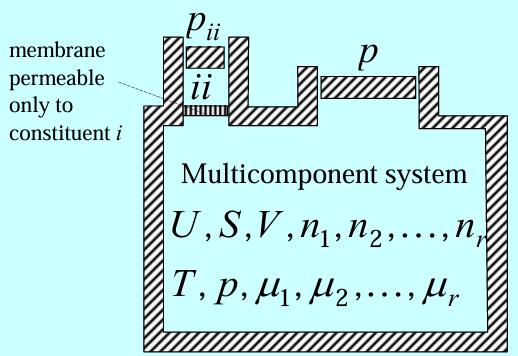
\includegraphics[width=\linewidth]{chap1/image/5.1.png}
    \end{minipage}
    \begin{minipage}{0.45\textwidth}
        \vspace*{0pt} 
        \parbox[t]{\linewidth}{ 
            Mutual stable equilibrium across the semi-permeable membrane implies:
            \begin{gather*}
                T = T_{ii}\\
                \mu_i(T,p,\vec{n})=\mu_{ii}(T,p_{ii})
            \end{gather*}
            This measurement procedure defines \textbf{the partial pressure} of constituent \(i\) in the mixture.
        }
    \end{minipage}

    \textcolor{b1}{注:}A \href{https://www.zhihu.com/question/26131215/answer/32303725}{membrane} is a selective barrier at times 
    it is also a outer covering of cell or cell organelle that allows 
    the passage of certain constituents and 
    retains other constituents found in the liquid.

\fbox{  
    \parbox{0.9\linewidth}{\centering
        the chemical potential of pure constituent \(i\) as function of
        temperature and pressure\\
        evaluating it at the temperature and
        \(\quad\Downarrow\quad\)
        partial pressure of the mixture\\
        the chemical potential of the constituent \(i\) in the mixture}}
\end{example}
\begin{add}
    Summary of propertie
    \begin{center} 
        \begin{minipage}{0.45\textwidth}
        \centering
        \begin{tabular}{|c|}
        \hline
        \textbf{Properties Defined for All States} \\
        \textbf{(Including SES and NEs)} \\ \hline
        Energy \(E\) \\ \hline
        Entropy \(S\) \\ \hline
        Volume \(V\) \\ \hline
        Amounts of constituents \(\vec{n}\) \\ \hline
        Availabilities \\ \hline
        \end{tabular}
        \end{minipage}
        \hfil
        \begin{minipage}{0.45\textwidth}
        \centering
        \begin{tabular}{|c|}
        \hline
        \textbf{Properties Defined Only for SES} \\
        \textbf{(All of Them)} \\ \hline
        Temperature \(T\) \\ \hline
        Pressure \(P\) \\ \hline
        Chemical potentials \(\vec{\mu}\) \\ \hline
        Enthalpy \(H\) \\ \hline
        Gibbs free energy \(G\) \\ \hline
        \end{tabular}
        \end{minipage}
        
        \begin{minipage}{0.7\textwidth}
        \centering
        \begin{tabular}{|c|}
        \hline
        \textbf{Properties Defined Only for Some SES} \\
        \textbf{(e.g. Not for Two-phase States)} \\ \hline
        Specific heat at constant volume \(C_v\) \\ \hline
        Specific heat at constant pressure \(C_p\) \\ \hline
        Isobaric expansion coefficient \(\alpha_p\) \\ \hline
        Isothermal compressibility coefficient \(\kappa_T\) \\ \hline
        \end{tabular}
        \end{minipage}
\end{center}
\end{add}
\begin{thm}
    Legendre Transform of a Function of a Single Variable

Consider a curve described by the convex or concave monotonic function:
\[
F = F(y), \quad \lambda(y) = \frac{\partial F}{\partial y}, \quad L(y) = F(y) - \lambda(y)y
\]
We can describe the same curve also as the envelope of the family of its tangent lines.

Since \(F(y)\) is convex or concave and monotonic, 
\(\lambda = \lambda(y)\) is monotonic and hence invertible. 
Using its inverse, \(y = y(\lambda)\), we find the Legendre transform of \(F = F(y)\):
\begin{gather*}
    L = L(\lambda) = F(y(\lambda)) - \lambda y(\lambda)
    \\
    \eta(\lambda) = \frac{\partial L}{\partial \lambda} 
    = \frac{\partial F}{\partial y} \frac{\partial y}{\partial \lambda} 
    - y(\lambda) - \lambda \frac{\partial y}{\partial \lambda} 
    = -y(\lambda)\quad \Rightarrow\quad \eta = -y
    \\
    G = G(\eta) = L(\lambda(\eta)) - \eta \lambda(\eta)
    \\
    G(y) = G(-\eta) = L(\lambda(y)) + y \lambda(y) 
    = F(y(\lambda(y))) - \lambda(y) y(\lambda(y)) + y \lambda(y) = F(y)
\end{gather*}
\end{thm}

\ifx\allfiles\undefined
\documentlecture[12pt, a4paper, oneside, UTF8]{ctexbook}  %  这一句是新增加的
\usepackage[dvipsnames]{xcolor}
\usepackage{amsmath}   % 数学公式
\usepackage{graphicx}
\usetikzlibrary{arrows, calc, decorations.pathmorphing}
\allowdisplaybreaks % 允许公式跨页换行
\newcommand{\pa}{\partial}
\newcommand{\mathminus}{\!\!-\!\!} % 数学环境连字符
\newcommand{\vsup}[1]{\raisebox{-0.1ex}{$\scriptstyle #1$}}
\newcommand{\lsup}[1]{\raisebox{-0.85ex}{$\scriptstyle #1$}}
\definecolor{b1}{RGB}{0,191,255}



\begin{document}
%
 % 单独编译时,其实不用编译封面目录之类的,如需要不注释这句即可
\else
\fi
%  ↓↓↓↓↓↓↓↓↓↓↓↓↓↓↓↓↓↓↓↓↓↓↓↓↓↓↓↓ 正文部分
\section{偏微分形式的热力学恒等式}
本节为补充内容,相关推导过程参考了知乎用户 \href{https://zhuanlan.zhihu.com/p/622282265}{Harogenshi} 
和 \href{https://zhuanlan.zhihu.com/p/115068655}{mosekyo} 的文章,特此致谢。

\begin{lemma}
    体积膨胀系数\(\alpha_p\),定温圧缩系数\(\kappa_T\),等熵(绝热)压缩系数\(\kappa_S\)
    \begin{align*}
        \alpha_p &= \frac{1}{V} \left( \frac{\partial V}{\partial T} \right)_p \\
        \kappa_T &= -\frac{1}{V} \left( \frac{\partial V}{\partial p} \right)_T
        =-\left(\frac{\partial \ln V}{\partial p}\right)_T \\
        \kappa_S &= -\frac{1}{V} \left( \frac{\partial V}{\partial p} \right)_S
    \end{align*}
\end{lemma}
\begin{lemma}
\begin{itemize}
    偏导数之间的运算规则
    \item 倒数法则 (INV)
    \[
    \left( \frac{\partial X}{\partial Y} \right)_Z \left( \frac{\partial Y}{\partial X} \right)_Z = 1
    \]    
    \item 三元轮换法则 (TRI)
    \[
    \left( \frac{\partial X}{\partial Y} \right)_Z \left( \frac{\partial Y}{\partial Z} \right)_X \left( \frac{\partial Z}{\partial X} \right)_Y = -1
    \]
    \item 复合法则 (CP)
    \[
    \left( \frac{\partial X}{\partial Y} \right)_Z = \left( \frac{\partial X}{\partial A} \right)_B \left( \frac{\partial A}{\partial Y} \right)_Z + \left( \frac{\partial X}{\partial B} \right)_A \left( \frac{\partial B}{\partial Y} \right)_Z
    \]
    \begin{itemize}
        \item  (CP1 \( B = Z \) )
        \[
        \left( \frac{\partial X}{\partial Y} \right)_Z = \left( \frac{\partial X}{\partial A} \right)_Z \left( \frac{\partial A}{\partial Y} \right)_Z
        \]
        \item  (CP2 \( B = Y \) )
        \[
        \left( \frac{\partial X}{\partial Y} \right)_Z =  
        \left( \frac{\partial X}{\partial A} \right)_Y \left( \frac{\partial A}{\partial Y} \right)_Z
        +\left( \frac{\partial X}{\partial Y} \right)_A
        \]
    \end{itemize}
\end{itemize}
\end{lemma}
\begin{corollary}
    用大写字母表示
\(E or U\)、
\(H\)、
\(S\)、
\(A or F\)、
\(G\),用小写字母表示
\(p\)、
\(V\)、
\(T\)。
    \begin{itemize}
        \item \[
        \left(\frac{\pa b }{\pa a}\right)_Z=-\frac{1}
        {\left(\frac{\pa a}{\pa Z}\right)_b\left(\frac{\pa Z}{\pa b}\right)_a}
        =-\frac{\left(\frac{\pa Z}{\pa a}\right)_b}{\left(\frac{\pa Z}{\pa b}\right)_a}\]
        \item \[
        \left(\frac{\pa X}{\pa Y}\right)_a=\left(\frac{\pa X}{\pa b}\right)_a 
        \left(\frac{\pa b}{\pa Y}\right)_a 
        =\frac{\left(\frac{\pa X}{\pa b}\right)_a }
        {\left(\frac{\pa Y}{\pa b}\right)_a }\]
        \item \[
        \left(\frac{\pa X}{\pa a}\right)_Y =\left(\frac{\pa X}{\pa a}\right)_b 
        +\left(\frac{\pa X}{\pa b}\right)_a\left(\frac{\pa b}{\pa a}\right)_Y
        =\left(\frac{\pa X}{\pa a}\right)_b 
        +\left(\frac{\pa X}{\pa b}\right)_a
        -\frac{\left(\frac{\pa Y}{\pa a}\right)_b}{\left(\frac{\pa Y}{\pa b}\right)_a}\]
        \item 
\begin{align*}
            \left(\frac{\pa X}{\pa Y}\right)_Z 
            &=\left( \frac{\partial X}{\partial a} \right)_Z \left( \frac{\partial a}{\partial Y} \right)_Z\\
            &=\left(\left(\frac{\pa X}{\pa a}\right)_b 
            +\left(\frac{\pa X}{\pa b}\right)_a
            -\frac{\left(\frac{\pa Z}{\pa a}\right)_b}{\left(\frac{\pa Z}{\pa b}\right)_a} \right)
            \left( \frac{1}{
                \left(\frac{\pa Y}{\pa a}\right)_b 
        +\left(\frac{\pa Y}{\pa b}\right)_a
        -\frac{\left(\frac{\pa Z}{\pa a}\right)_b}{\left(\frac{\pa Z}{\pa b}\right)_a}
            }\right)
\end{align*}
            \begin{center}
                \includegraphics*[width=0.4\textwidth]{chap1/image/eq.1.jpg}
            \end{center}
            综合上述公式,我们可以把所有的偏微分关系式化成一阶的关系式
            \(\left(\frac{\pa X}{\pa a}\right)_b\)
    \end{itemize}
\end{corollary}
\begin{example}
    \(U\)的偏微分关系
    \begin{enumerate}
        \item \[\left(\frac{\pa U}{\pa T}\right)_V =C_V
        \]
        \hrule
        \item\label{1.2} \[\left(\frac{\pa U}{\pa p}\right)_V
        \overset{CP1}{=}\left(\frac{\pa U}{\pa T}\right)_V\left(\frac{\pa T}{\pa p}\right)_V
        =C_V\left(\frac{\pa T}{\pa p}\right)_V
        \]
        \hrule
        \item\label{1.3} \begin{align*}
            \left(\frac{\pa U}{\pa T}\right)_p
            =\left(\frac{\pa H}{\pa T}\right)_p
            -p\left(\frac{\pa H}{\pa T}\right)_p
            &=C_p -p\left(\frac{\pa V}{\pa T}\right)_p\\
            &=C_p -pV\alpha_p
        \end{align*}
        \hrule
        \item\label{1.4} \[\left(\frac{\pa U}{\pa V}\right)_p=
        \left(\frac{\pa U}{\pa T}\right)_p\left(\frac{\pa T}{\pa V}\right)_p
        \overset{\ref*{1.3}}{=}
        C_p \left(\frac{\pa T}{\pa V}\right)_p-p\left(\frac{\pa V}{\pa T}\right)_p\left(\frac{\pa T}{\pa V}\right)_p
        =C_p \left(\frac{\pa T}{\pa V}\right)_p-p
        \]
        \hrule
        \item\label{1.5} \begin{align*}
            \left(\frac{\pa U}{\pa V}\right)_T 
            &\overset{CP2}{=}\left(\frac{\pa U}{\pa V}\right)_p+
            \left(\frac{\pa U}{\pa p}\right)_V\left(\frac{\pa p}{\pa V}\right)_T\\
            &\overunderset{\ref*{1.2}}{\ref*{1.4}}{=}
            C_p\left(\frac{\pa T}{\pa V}\right)_p-p+C_V 
            \left(\frac{\pa T}{\pa p}\right)_V\left(\frac{\pa p}{\pa V}\right)_T \\
            &\overset{TRI}{=}C_p\left(\frac{\pa T}{\pa V}\right)_p-p -C_V 
            \left(\frac{\pa T}{\pa V}\right)_p \\
            &=(C_p-C_V)\left(\frac{\pa T}{\pa V}\right)_p-p
        \end{align*}
        \hrule
        \item \begin{align*}
            \left(\frac{\pa U}{\pa p}\right)_T
            \overset{INV}{=}\left(\frac{\pa U}{\pa V}\right)_T\left(\frac{\pa V}{\pa p}\right)_T
            &\overunderset{\ref*{1.5}}{TRI}{=}
            -(C_p-C_V)\left(\frac{\pa T}{\pa p}\right)_V-p\left(\frac{\pa V}{\pa p}\right)_T\\
            &= -T \alpha_pV \left( \frac{\partial p}{\partial T} \right)_V \left(\frac{\pa T}{\pa p}\right)_V
            -p\left(\frac{\pa V}{\pa p}\right)_T
            \\&\overset{INV}{=}(p\kappa_T -T \alpha_p)V
        \end{align*}
    \end{enumerate}
\end{example}
\begin{example}
    \( H \) 的偏微分关系
    \begin{enumerate}
        \item \[\left(\frac{\partial H}{\partial T}\right)_p = C_p \]
        \hrule
        \item\label{2.2} \[\left(\frac{\partial H}{\partial V}\right)_p 
        \overset{CP1}{=} \left(\frac{\partial H}{\partial T}\right)_p \left(\frac{\partial T}{\partial V}\right)_p 
        = C_p \left(\frac{\partial T}{\partial V}\right)_p 
        \]
        \hrule
        \item\label{2.3} \begin{align*}
        \left(\frac{\partial H}{\partial p}\right)_T 
        = \left(\frac{\partial U}{\partial p}\right)_T 
        + \left(\frac{\partial (pV)}{\partial p}\right)_T 
        &= \left(\frac{\partial U}{\partial p}\right)_T 
        + V + p\left(\frac{\partial V}{\partial p}\right)_T \\
        &=V-(C_p-C_V)\left(\frac{\pa T}{\pa p}\right)_V\\
        &=V-T \alpha_pV \left( \frac{\partial p}{\partial T} \right)_V
        \left(\frac{\pa T}{\pa p}\right)_V \overset{INV}{=}(1-T \alpha_p)V
        \end{align*}
        \hrule
        \item\label{2.4} \begin{align*}
            \left(\frac{\partial H}{\partial T}\right)_V 
            \overset{CP2}{=} \left(\frac{\partial H}{\partial T}\right)_p 
            + \left(\frac{\partial H}{\partial p}\right)_T \left(\frac{\partial p}{\partial T}\right)_V 
            &\overset{\ref*{2.3}}{=} C_p + \left[ V 
            + p\left(\frac{\partial V}{\partial p}\right)_T \right]
            \left(\frac{\partial p}{\partial T}\right)_V \\
            &=C_V + V\left(\frac{\pa p}{\pa T}\right)_V
        \end{align*}
        \hrule
        \item\label{2.5} \begin{align*}
            \left(\frac{\partial H}{\partial V}\right)_T 
            &\overset{CP2}{=} \left(\frac{\partial H}{\partial V}\right)_p 
            + \left(\frac{\partial H}{\partial p}\right)_V \left(\frac{\partial p}{\partial V}\right)_T \\
            &\overunderset{\ref*{2.2}}{\ref*{2.3}}{=} 
            C_p \left(\frac{\partial T}{\partial V}\right)_p 
            + \left[ V + p\left(\frac{\partial V}{\partial p}\right)_T \right] 
            \left(\frac{\partial p}{\partial V}\right)_T \\
            &\overset{TRI}{=}V\left(\frac{\partial p}{\partial V}\right)_T
            +(C_p-C_V)\left(\frac{\partial T}{\partial V}\right)_p
        \end{align*}
        \hrule
        \item \begin{align*}
            \left(\frac{\partial H}{\partial p}\right)_V 
            \overset{CP1}{=} \left(\frac{\partial H}{\partial T}\right)_V 
            \left(\frac{\partial T}{\partial p}\right)_V 
            &\overset{\ref*{2.4}}{=} 
            \left[ C_p + \left( V + p\left(\frac{\partial V}{\partial p}\right)_T \right) 
            \left(\frac{\partial p}{\partial T}\right)_V \right] 
            \left(\frac{\partial T}{\partial p}\right)_V \\
            &=C_V + V\left(\frac{\pa p}{\pa T}\right)_V
        \end{align*}
    \end{enumerate}
\end{example}
\begin{example}
    \( S \) 的偏微分关系
    \begin{enumerate}
        \item\label{3.1} \[\left(\frac{\partial S}{\partial T}\right)_V 
        =\left(\frac{\pa S}{\pa U}\right)_V\left(\frac{\pa U}{\pa T}\right)_V
        = \frac{C_V}{T} 
        \]\hrule
        \item\label{3.2} \[\left(\frac{\partial S}{\partial T}\right)_p 
        =\left(\frac{\pa S}{\pa H}\right)_p\left(\frac{\pa H}{\pa T}\right)_p
        = \frac{C_p}{T} 
        \]\hrule
        \item\label{3.3} \[\left(\frac{\partial S}{\partial V}\right)_T 
        \overset{\text{Maxwell}}{=} \left(\frac{\partial p}{\partial T}\right)_V \quad (\text{由}  dA = -S dT - p dV ) \]
        \hrule
        \item\label{3.4} \[\left(\frac{\partial S}{\partial p}\right)_T 
        \overset{\text{Maxwell}}{=} -\left(\frac{\partial V}{\partial T}\right)_p \quad (\text{由}  dG = -S dT + V dp ) \]
        \hrule
        \item\label{3.5} \begin{align*}
            \left(\frac{\partial S}{\partial V}\right)_p 
            \overset{CP1}{=} \left(\frac{\partial S}{\partial T}\right)_p \left(\frac{\partial T}{\partial V}\right)_p
            \overunderset{\ref*{3.2}}{\ref*{3.3}}{=} 
            \frac{C_p}{T} \left(\frac{\partial T}{\partial V}\right)_p  
        \end{align*}
        \hrule
        \item\label{3.6} \begin{align*}
            \left(\frac{\partial S}{\partial p}\right)_V 
            \overset{CP1}{=} \left(\frac{\partial S}{\partial T}\right)_V \left(\frac{\partial T}{\partial p}\right)_V
            \overunderset{\ref*{3.1}}{\ref*{3.4}}{=} 
            \frac{C_V}{T} \left(\frac{\partial T}{\partial p}\right)_V
        \end{align*}
    \end{enumerate}
\end{example}
\begin{example}
    \( A \) 的偏微分关系
    \begin{enumerate}
        \item\label{4.1} \[\left(\frac{\partial A}{\partial T}\right)_V = -S \quad (\text{由} \ dA = -S dT - p dV ) \]
        \hrule
        \item\label{4.2} \[\left(\frac{\partial A}{\partial V}\right)_T = -p \quad (\text{由} \ dA = -S dT - p dV ) \]
        \hrule
        \item\label{4.3} \begin{align*}
            \left(\frac{\partial A}{\partial p}\right)_V 
            \overset{CP1}{=} \left(\frac{\partial A}{\partial T}\right)_V 
            \left(\frac{\partial T}{\partial p}\right)_V 
            \overset{\ref*{4.1}}{=} -S \left(\frac{\partial T}{\partial p}\right)_V
        \end{align*}
        \hrule
        \item\label{4.4} \begin{align*}
            \left(\frac{\partial A}{\partial p}\right)_T 
            \overset{CP1}{=} \left(\frac{\partial A}{\partial V}\right)_T 
            \left(\frac{\partial V}{\partial p}\right)_T 
            \overset{\ref*{4.2}}{=} -p \left(\frac{\partial V}{\partial p}\right)_T
        \end{align*}
        \hrule
        \item\label{4.5} \begin{align*}
            \left(\frac{\partial A}{\partial T}\right)_p 
            &\overset{CP2}{=} \left(\frac{\partial A}{\partial T}\right)_V 
            + \left(\frac{\partial A}{\partial V}\right)_T 
            \left(\frac{\partial V}{\partial T}\right)_p \\
            &\overunderset{\ref*{4.1}}{\ref*{4.2}}{=} -S -p \left(\frac{\partial V}{\partial T}\right)_p
        \end{align*}
        \hrule
        \item\label{4.6} \begin{align*}
            \left(\frac{\partial A}{\partial T}\right)_p 
            &\overset{CP2}{=} \left(\frac{\partial A}{\partial T}\right)_V 
            \left(\frac{\partial T}{\partial V}\right)_p
            + \left(\frac{\partial A}{\partial V}\right)_T  \\
            &\overunderset{\ref*{4.1}}{\ref*{4.2}}{=} 
            -S\left(\frac{\partial T}{\partial V}\right)_p -p 
        \end{align*}
    \end{enumerate}
\end{example}
\begin{example}
    \( G \) 的偏微分关系
    \begin{enumerate}
        \item\label{5.1} \[\left(\frac{\partial G}{\partial T}\right)_p = -S \quad (\text{由} \ dG = -S dT + V dp ) \]
        \hrule
        \item\label{5.2} \[\left(\frac{\partial G}{\partial p}\right)_T = V \quad (\text{由} \ dG = -S dT + V dp ) \]
        \hrule
        \item\label{5.3} \begin{align*}
            \left(\frac{\partial G}{\partial V}\right)_P 
            \overset{CP1}{=} \left(\frac{\partial G}{\partial T}\right)_p 
            \left(\frac{\partial T}{\partial V}\right)_p 
            \overset{\ref*{5.1}}{=} -S \left(\frac{\partial p}{\partial V}\right)_T
        \end{align*} 
        \hrule
        \item\label{5.4} \begin{align*}
            \left(\frac{\partial G}{\partial V}\right)_T 
            \overset{CP1}{=} \left(\frac{\partial G}{\partial p}\right)_T 
            \left(\frac{\partial p}{\partial V}\right)_T 
            \overset{\ref*{5.2}}{=} V \left(\frac{\partial p}{\partial V}\right)_T
        \end{align*}
        \hrule
        \item\label{5.5} \begin{align*}
            \left(\frac{\partial G}{\partial T}\right)_V 
            &\overset{CP2}{=} \left(\frac{\partial G}{\partial T}\right)_p 
            + \left(\frac{\partial G}{\partial p}\right)_T 
            \left(\frac{\partial p}{\partial T}\right)_V \\
            &\overunderset{\ref*{5.1}}{\ref*{5.2}}{=} 
            -S + V \left(\frac{\partial p}{\partial T}\right)_V
        \end{align*}
        \hrule
        \item\label{5.6} \begin{align*}
            \left(\frac{\partial G}{\partial T}\right)_V 
            &\overset{CP2}{=} \left(\frac{\partial G}{\partial T}\right)_p 
            \left(\frac{\partial T}{\partial p}\right)_V
            + \left(\frac{\partial G}{\partial p}\right)_T \\
            &\overunderset{\ref*{5.1}}{\ref*{5.2}}{=} 
            -S\left(\frac{\partial T}{\partial p}\right)_V + V 
        \end{align*}
    \end{enumerate}
\end{example}

















%  ↑↑↑↑↑↑↑↑↑↑↑↑↑↑↑↑↑↑↑↑↑↑↑↑↑↑↑↑ 正文部分
\ifx\allfiles\undefined
\end{document}
\fi
\label{eq.tex}

\section{lecture 6}
\begin{minipage}{0.9\linewidth}
        \centering
        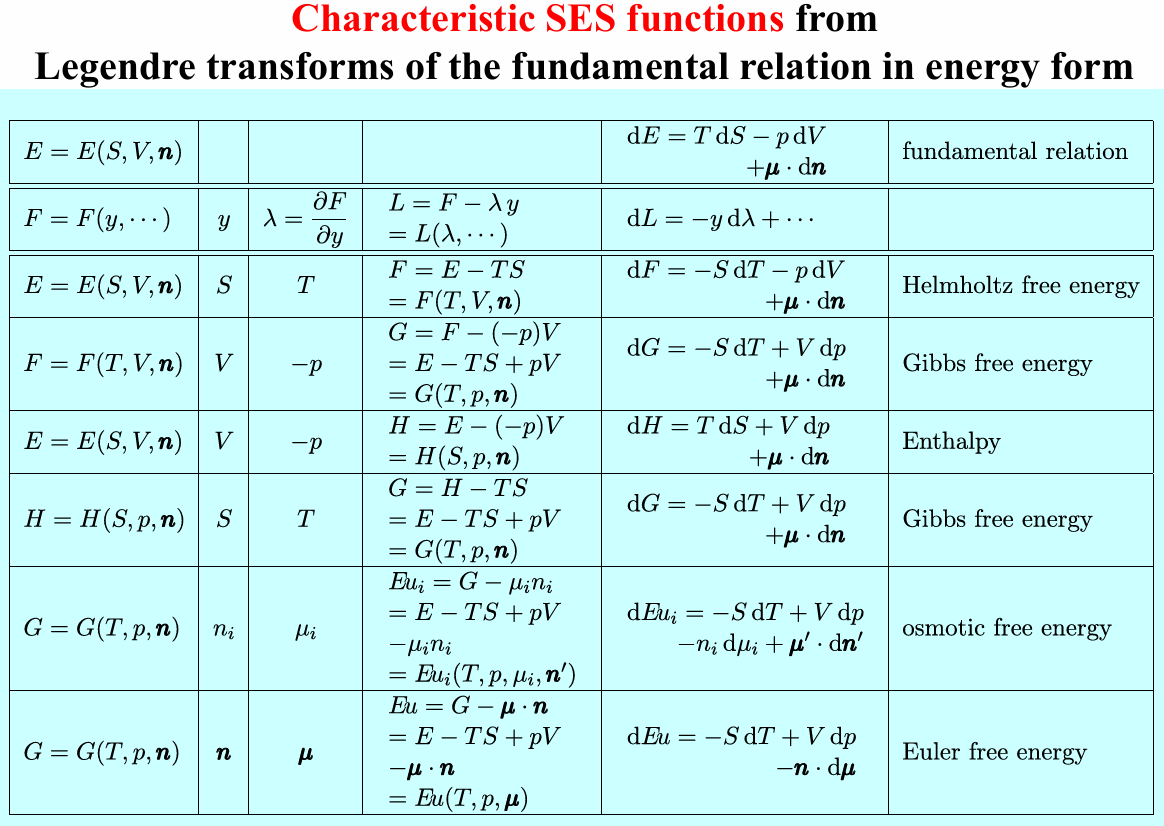
\includegraphics[scale=0.45]{chap1/image/6.1.png}
        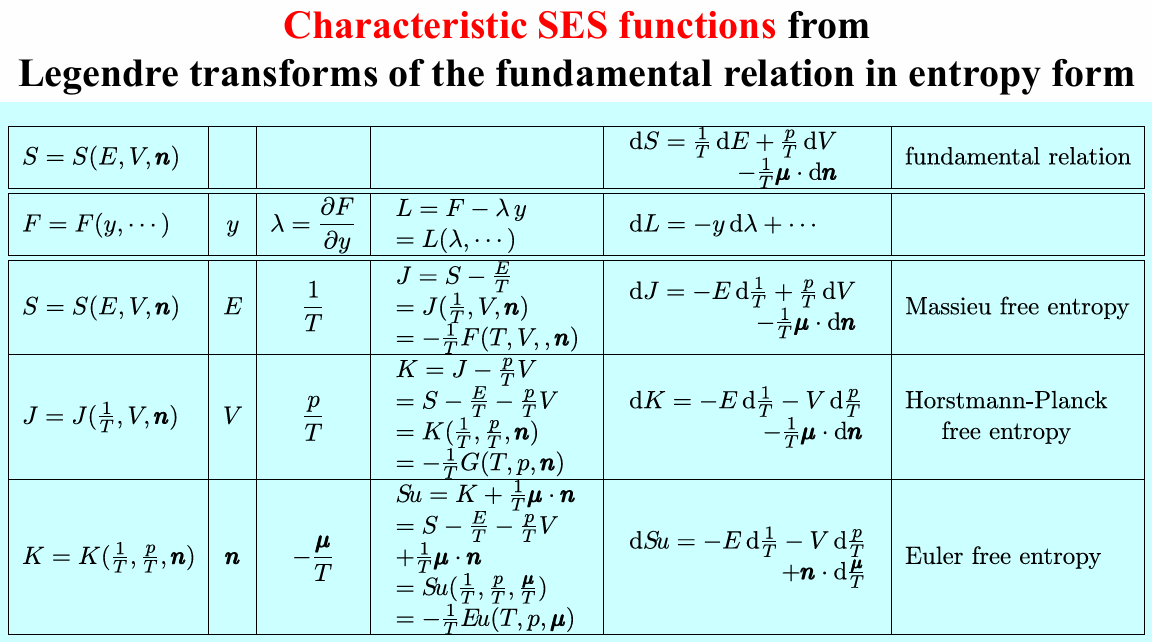
\includegraphics[scale=0.45]{chap1/image/6.2.png}
\end{minipage}
\begin{thm}
    Stability conditions deriving from the available energy \textbf{(with fixed volume and amounts)}

    The canonical availability function \( \Gamma \) is:
\[
\Gamma = E - T_R S
\]

If \( A \) is in state \( A_R \) (MSE with the thermal reservoir \( R \)), any variation to another state \( A_1 \) satisfies:
\[
\Delta \Gamma^A = \Gamma_1^A - \Gamma_R^A > 0
\]
\begin{itemize}
    \item For \textbf{a neighboring SES} with \( \Delta S^A = dS \) and constant \( V \) and \( n \):
\[
\Delta E^A = E^A(S_R + dS, V, n) - E_R^A = T_R dS + \frac{1}{2}d^2E^A|_{V,n} + \cdots
\]

This implies:
\[
\Delta \Gamma^A = \Delta E^A - T_R \Delta S^A = \frac{1}{2}d^2E^A|_{V,n} + \cdots > 0 \Rightarrow d^2E^A|_{V,n} > 0
\]

\item Alternatively, for \textbf{a neighboring SES} with \( \Delta E^A = dE \) and constant \( V \) and \( n \):
\[
\Delta S^A = S^A(E_R + dE, V, n) - S_R^A = \frac{1}{T_R}dE + \frac{1}{2}d^2S^A|_{V,n} + \cdots
\]

This implies:
\[
\Delta \Gamma^A = \Delta E^A - T_R \Delta S^A = -\frac{1}{2}d^2S^A|_{V,n} + \cdots > 0 \Rightarrow d^2S^A|_{V,n} < 0
\]
\end{itemize}
\begin{zhu}
    这里Beretta教授在幻灯片上写的是\(d^2E^A|_{V,n} \geq 0\),\(d^2S^A|_{V,n} \leq 0\),等号只在相平衡等特殊情况下取得。
    多数情况都取严格不等号,跟之前第\pageref{<>}页的原因类似。一般化的表达式见原理\ref{l-bp}
    
    这里我想到了另一个更数学的解释,一阶导数为零,为了保证一定取极值,二阶导数严格大于(小于)零。
    否则有可能第一个非零导数为奇数阶,无极值,与
    Minimum energy principle和Maximum entropy principle矛盾。
\end{zhu}
\end{thm}
\section{lecture 7}
\begin{defn}
    Jacobian (determinants)
\begin{align*}
\frac{\partial (f,g)}{\partial (x,y)} 
= \left| \begin{array}{cc} 
\left( \frac{\partial f}{\partial x} \right)_y & \left( \frac{\partial f}{\partial y} \right)_x \\ 
\left( \frac{\partial g}{\partial x} \right)_y & \left( \frac{\partial g}{\partial y} \right)_x 
\end{array} \right| 
= - \frac{\partial (g,f)}{\partial (x,y)} 
= \frac{\partial (g,f)}{\partial (y,x)} 
= - \frac{\partial (f,g)}{\partial (y,x)}
\end{align*}
\end{defn}

\begin{example}
    第\pageref{kappa_s}页的恒等式的一种更简便的推导方法
    \begin{align*}
    \det(\text{Hess}(E)) &= 
    \begin{vmatrix}
    \frac{\partial^2 E}{\partial S^2} & \frac{\partial^2 E}{\partial S \partial V} \\
    \frac{\partial^2 E}{\partial V \partial S} & \frac{\partial^2 E}{\partial V^2}
    \end{vmatrix}
    = 
    \begin{vmatrix}
    \left( \frac{\partial T}{\partial S} \right)_V & -\left( \frac{\partial p}{\partial S} \right)_V \\
    \left( \frac{\partial T}{\partial V} \right)_S & -\left( \frac{\partial p}{\partial V} \right)_S
    \end{vmatrix}
    = -\frac{\partial(T,p)}{\partial(S,V)} 
    \\&= 
    \begin{cases}
    -\frac{\partial(T,p)}{\partial(S,p)} \frac{\partial(S,p)}{\partial(S,V)} 
    =- \left( \frac{\partial T}{\partial S} \right)_p 
    \left( \frac{\partial p}{\partial V} \right)_S 
    = \frac{T}{C_p} \frac{1}{V \kappa_S} \geq 0 \\
    -\frac{\partial(T,p)}{\partial(T,V)} \frac{\partial(T,V)}{\partial(S,V)} 
    =- \left( \frac{\partial p}{\partial V} \right)_T 
    \left( \frac{\partial T}{\partial S} \right)_V 
    = \frac{1}{V \kappa_T} \frac{T}{C_V} \geq 0
    \end{cases}
    \Rightarrow 
     \frac{C_p}{C_V} = \frac{\kappa_T}{\kappa_S}
    \end{align*}
    \begin{explain}
    第一个等式的雅可比行列式计算
\begin{align*}
        \frac{\partial(T,p)}{\partial(S,p)} = 
        \begin{vmatrix}
        \left( \frac{\partial T}{\partial S} \right)_p & \left( \frac{\partial T}{\partial p} \right)_S \\
        \left( \frac{\partial p}{\partial S} \right)_p & \left( \frac{\partial p}{\partial p} \right)_S
        \end{vmatrix}
        &= \left( \frac{\partial T}{\partial S} \right)_p - \left( \frac{\partial T}{\partial p} \right)_S \left( \frac{\partial p}{\partial S} \right)_p
        =\left( \frac{\partial T}{\partial S} \right)_p\\
        \frac{\partial(S,p)}{\partial(S,V)} &= 
        \begin{vmatrix}
        \left( \frac{\partial S}{\partial S} \right)_V & \left( \frac{\partial S}{\partial V} \right)_S \\
        \left( \frac{\partial p}{\partial S} \right)_V & \left( \frac{\partial p}{\partial V} \right)_S
        \end{vmatrix}
        = \left( \frac{\partial p}{\partial V} \right)_S
        \\
-\frac{\partial(T,p)}{\partial(S,p)} \frac{\partial(S,p)}{\partial(S,V)} 
&= -\left( \frac{\partial T}{\partial S} \right)_p \left( \frac{\partial p}{\partial V} \right)_S
\end{align*}
    
    第二个等式的雅可比行列式计算
\begin{align*}
        \frac{\partial(T,p)}{\partial(T,V)} &= 
        \begin{vmatrix}
        \left( \frac{\partial T}{\partial T} \right)_V & \left( \frac{\partial T}{\partial V} \right)_T \\
        \left( \frac{\partial p}{\partial T} \right)_V & \left( \frac{\partial p}{\partial V} \right)_T
        \end{vmatrix}
        = \left( \frac{\partial p}{\partial V} \right)_T
        \\
        \frac{\partial(T,V)}{\partial(S,V)} &= 
        \begin{vmatrix}
        \left( \frac{\partial T}{\partial S} \right)_V & \left( \frac{\partial T}{\partial V} \right)_S \\
        \left( \frac{\partial V}{\partial S} \right)_V & \left( \frac{\partial V}{\partial V} \right)_S
        \end{vmatrix}
        = \left( \frac{\partial T}{\partial S} \right)_V
        \\ 
        -\frac{\partial(T,p)}{\partial(T,V)} \frac{\partial(T,V)}{\partial(S,V)} 
&= -\left( \frac{\partial p}{\partial V} \right)_T \left( \frac{\partial T}{\partial S} \right)_V
\end{align*}
    \end{explain}
\end{example}
\begin{example}\label{proofTRI}
    Prove cyclic relation (\pageref{TRI}) using Jacobians

    the three functions
\(\begin{cases}
x = x(y, z) \\
y = y(z, x) \\
z = z(x, y)
\end{cases}\)
which represent the same surface \( f(x, y, z) = 0 \). 
\[    \frac{\partial(x,z)}{\partial(y,z)}\frac{\partial(y,x)}{\partial(z,x)}\frac{\partial(z,y)}{\partial(x,y)} 
    = \frac{\overbrace{\partial(x,z)}^{-1}}{\partial(z,x)}
    \frac{\overbrace{\partial(y,x)}^{-1}}{\partial(x,y)}
    \frac{\overbrace{\partial(z,y)}^{-1}}{\partial(y,z)}
    =\left(-\frac{\partial(x,z)}{\partial(z,y)}\right) 
    \left(-\frac{\partial(y,x)}{\partial(x,z)}\right) 
    \left(-\frac{\partial(z,y)}{\partial(y,x)}\right)
    = -1\]
\end{example}
\begin{principle}\label{l-bp}
    LeChatelier-Braun principle
\begin{gather*}
    \left( \frac{\partial^2 S}{\partial E^2} \right)_{n,V} \leq 0 \Rightarrow \left( \frac{\partial T}{\partial E} \right)_{n,V} \geq 0
    \\
    \left( \frac{\partial^2 E}{\partial S^2} \right)_{n,V}^A \geq 0 \Rightarrow \left( \frac{\partial T}{\partial S} \right)_{n,V} \geq 0
\end{gather*}
\begin{zhu}
    更一般的形式见原理\ref{l-bpg}
\end{zhu}
\begin{zhu}
    通常在以下场景,等号成立:
\begin{itemize}
    \item \textbf{稳定性边界}:系统处于稳定与不稳定的临界点,热力学势的二阶导数为零;
    \item \textbf{相变现象}:在二级相变(指相变过程中热力学势的一阶导数连续,但二阶导数不连续或发散的相变。)
    的临界点,响应函数(热容、压缩率、磁化率等)趋于零或发散;
    \item \textbf{理想化极限}:完全均质或无相互作用的系统可能严格满足等式。
\end{itemize}
\end{zhu}
\end{principle}
\begin{thm}
    Stability conditions deriving from the available energy 
    \textbf{(with changes in \textcolor{b1}{variable amount} of “i” at fixed volume)}

If \( A \) is in state \( A_R \) (MSE with the thermal reservoir \( R \)), any possible variation to another state \( A_1 \) is such that  
\[
\Delta \Upsilon^A = \Upsilon_1^A - \Upsilon_R^A > 0 \quad \text{where} \quad \Upsilon^A = E^A - T_R S^A - \mu_i n_i^A
\]  
choose \( A_1 \) to be the neighbouring SES with \(\Delta S^A = dS\), 
\(\Delta n_i^A = dn_i\) and the same values of \( V \) and 
the other \( n_i' \), so that  
\begin{gather*}
    \Delta E^A = E^A(S_R + dS, V, n_{iR} + dn_i, n_i') - E_R^A 
    = T_R dS + \mu_{iR }+ \frac{1}{2} d^2 E^A |_{V, n_i'} + \cdots
    \\
    \Delta \Upsilon^A = \Delta E^A - T_R \Delta S^A - \mu_i n_i^A 
    = \frac{1}{2} d^2 E^A |_{V, n_i'} + \cdots > 0 
    \quad \Rightarrow \quad d^2 E^A |_{V, n_i'} \geq 0
\end{gather*}
choose instead \( A_1 \) to be the neighbouring SES with \(\Delta E^A = dE\), 
\(\Delta n_i^A = dn_i\) and the same values of \( V \) and 
the other \( n_i' \), so that  
\begin{gather*}
    \Delta S^A = S^A(E_R + dE, V, n_{iR} + dn_i, n_i') - S_R^A 
    = \frac{1}{T_R} dE - \frac{\mu_{iR }}{T_R} dn_i 
    + \frac{1}{2} d^2 S^A |_{V, n_i'} + \cdots
    \\
    \Delta \Upsilon^A = \Delta E^A - T_R \Delta S^A + \mu_i n_i^A = -\frac{1}{2} d^2 S^A |_{V, n_i'} + \cdots > 0 \quad \Rightarrow \quad d^2 S^A |_{V, n_i'} \leq 0
\end{gather*}
\end{thm}
\begin{thm}
    Stability conditions deriving from the available energy \textbf{(with changes in \textcolor{b1}{volume} and amounts)}

    If \( A \) is in state \( A_R \) (MSE with the thermal reservoir \( R \)), any possible variation to another state \( A_1 \) is such that  
    \[
    \Delta \Xi^A = \Xi_1^A - \Xi_R^A > 0 \quad \text{where} \quad \Xi^A = E^A - T_R S^A + p_R V^A - \mu_R \cdot n^A
    \]  
    choose \( A_1 \) to be the neighbouring SES with \(\Delta S^A = dS\), \(\Delta V^A = dV\), and \(\Delta n_i^A = dn_i \forall i\), so that  
    \begin{gather*}
    \Delta E^A = E^A (S_R + dS, V_R + dV, \vec{n}_R + d\vec{n}) - E_R^A = T_R dS - p_R dV + \mu_R \cdot dn + \frac{1}{2} d^2 E^A + \cdots
    \\
    \Delta \Xi^A = \Delta E^A - T_R \Delta S^A + p_R \Delta V^A - \mu_R \cdot \Delta n^A = \frac{1}{2} d^2 E^A + \cdots > 0 \quad \Rightarrow \quad d^2 E^A \geq 0
    \end{gather*}
    choose instead \( A_1 \) to be the neighbouring SES with \(\Delta E^A = dE\), \(\Delta V^A = dV\), and \(\Delta n_i^A = dn_i \forall i\), so that  
\begin{align*}
        \Delta S^A &= S^A (E_R + dE, V_R + dV, \vec{n}_R + d\vec{n}) - S_R^A 
        \\
        &= \frac{1}{T_R} dE + \frac{p_R}{T_R} dV - \frac{1}{T_R} \mu_R \cdot dn + \frac{1}{2} d^2 S^A + \cdots
        \\
        \Delta \Xi^A &= \Delta E^A - T_R \Delta S^A + p_R \Delta V^A - \mu_R \cdot \Delta n^A = -\frac{1}{2} d^2 S^A + \cdots > 0 \quad \Rightarrow \quad d^2 S^A \leq 0
\end{align*}
\end{thm}
\begin{thm}
    Stability conditions deriving from the available energy with \textbf{(changes in the \textcolor{b1}{amounts} at fixed temperature and pressure)}

    If \( A \) is in state \( A_R \) (MSE with the thermal reservoir \( R \)), any possible variation to another state \( A_1 \) is such that  
    \[
    \Delta \Xi^A = \Xi_1^A - \Xi_R^A > 0 \quad \text{where} \quad \Xi^A = E^A - T_R S^A + p_R V^A - \mu_R \cdot n^A
    \]

    For example, choose \( A_1 \) to be the neighbouring SES with same temperature \( T_1^A = T_R \) and pressure \( p_1^A = p_R \), and \(\Delta n_i^A = dn_i \, \forall i\), so that  
\begin{gather*}
        \Delta E^A = E^A (T_R, p_R, \vec{n}_R + d\vec{n}) - E_R^A
    \\
        \Delta S^A = S^A (T_R, p_R, \vec{n}_R + d\vec{n}) - S_R^A
    \\
        \Delta V^A = V^A (T_R, p_R, \vec{n}_R + d\vec{n}) - V_R^A
\end{gather*}
\begin{align*}
        &\Delta E^A - T_R \Delta S^A + p_R \Delta V^A\\
        =& \Delta G^A = G^A (T_R, p_R, \vec{n}_R + d\vec{n}) - G_R^A = \mu_R \cdot dn + \frac{1}{2} d^2 G^A |_{T,p} + \cdots
    \\
        \Delta \Xi^A &= \Delta G^A - \mu_R \cdot \Delta n^A = \frac{1}{2} d^2 G^A |_{T,p} + \cdots > 0 \quad \Rightarrow \quad d^2 G^A |_{T,p} \geq 0
\end{align*}
\end{thm}
\begin{thm}
    Stability conditions deriving from the available energy with \textbf{(changes in \textcolor{b1}{volume and amounts} at fixed temperature)}

    If \( A \) is in state \( A_R \) (MSE with the thermal reservoir \( R \)), any possible variation to another state \( A_1 \) is such that  
    \[
    \Delta E^A = E_1^A - E_R^A > 0 \quad \text{where} \quad E^A = E^A - T_R S^A + p_R V^A - \mu_R \cdot n^A
    \]
    choose \( A_1 \) to be the neighbouring SES with same temperature \( T_1^A = T_R \), \(\Delta V^A = dV\), and \(\Delta n_i^A = dn_i \, \forall i\), so that  
    \[
    \Delta E^A = E^A(T_R, V_R + dV, \, \vec{n}_R + d\vec{n}) - E_R^A
    \]
    \[
    \Delta S^A = S^A(T_R, V_R + dV, \, \vec{n}_R + d\vec{n}) - S_R^A
    \]
\begin{align*}
    &\Delta E^A - T_R \Delta S^A\\
    =& \Delta F^A = F^A(T_R, V_R + dV, \, \vec{n}_R + d\vec{n}) - F_R^A = -p_R \, dV + \mu_R \cdot dn + \frac{1}{2} d^2 F^A |_T + \cdots
    \\
    \Delta E^A &= \Delta F^A + p_R \Delta V^A - \mu_R \cdot \Delta n^A = \frac{1}{2} d^2 F^A |_T + \cdots > 0 \quad \Rightarrow \quad d^2 F^A |_T \geq 0
\end{align*}
\end{thm}
\begin{principle}
    LeChatelier-Braun principle \textbf{(more general statement)}\label{l-bpg}
    \[
        \mathrm{d}^2A|_z\geq 0\Rightarrow
            \begin{cases}
                \left(\dfrac{\partial A_{x}}{\partial x}\right)_y
                \geq \left(\dfrac{\partial A_{x}}{\partial x}\right)_{A,y}\geq 0\\
                \left(\dfrac{\partial A_{y}}{\partial y}\right)_x
                \geq \left(\dfrac{\partial A_{y}}{\partial y}\right)_{A,x}\geq 0
            \end{cases}
        \hfil
        \mathrm{d}^2A|_z\leq 0\Rightarrow
        \begin{cases}\left(\dfrac{\partial A_{x}}{\partial x}\right)_y
            \leq \left(\dfrac{\partial A_{x}}{\partial x}\right)_{A,y}\leq 0\\
            \left(\dfrac{\partial A_{y}}{\partial y}\right)_x
            \leq \left(\dfrac{\partial A_{y}}{\partial y}\right)_{A,x}\leq 0
        \end{cases}
    \]
\begin{tui}
    Given a function \( A(x, y, z) \)
\begin{gather*}
        A_x = \left( \frac{\partial A}{\partial x} \right)_{y,z} = A_x(x, y, z) 
        \qquad A_y = \left( \frac{\partial A}{\partial y} \right)_{x,z} = A_y(x, y, z)
    \\
        A_{xx} = \left( \frac{\partial^2 A}{\partial x^2} \right)_{y,z} = \left( \frac{\partial A_x}{\partial x} \right)_{y,z} 
        \qquad A_{yy} = \left( \frac{\partial^2 A}{\partial y^2} \right)_{x,z} = \left( \frac{\partial A_y}{\partial y} \right)_{x,z}
    \\
        A_{xy} = \left( \frac{\partial^2 A}{\partial x\partial y} \right)_z = \left( \frac{\partial A_y}{\partial x} \right)_{y,z} = \left( \frac{\partial A_x}{\partial y} \right)_{x,z} = \left( \frac{\partial^2 A}{\partial y\partial x} \right)_z = A_{yx}
\end{gather*}  
\begin{align*}
        d^2A|_z &= A_{xx} \left( dx + \frac{A_{xy}}{A_{xx}} dy \right)^2 + \lambda_y (dy)^2 
        &\quad \text{where} \quad \lambda_y = A_{yy} - A_{xx} \left( \frac{A_{xy}}{A_{xx}} \right)^2
    \\
        &= \lambda_x (dx)^2 + A_{yy} \left( dy + \frac{A_{xy}}{A_{yy}} dx \right)^2 
        &\quad \text{where} \quad \lambda_x = A_{xx} - A_{yy} \left( \frac{A_{xy}}{A_{yy}} \right)^2
\end{align*}
    Therefore, since the stability conditions must hold for arbitrary \( dx \) and \( dy \),  
    \[
    d^2A|_z \geq 0 \Rightarrow 
        \begin{cases} A_{xx} \geq \lambda_x \geq 0 \\ 
        A_{yy} \geq \lambda_y \geq 0 \end{cases} 
        \quad \text{whereas} \quad 
        d^2A|_z \leq 0 \Rightarrow 
        \begin{cases} A_{xx} \leq \lambda_x \leq 0 \\ 
        A_{yy} \leq \lambda_y \leq 0 \end{cases}
    \]
Whether \( d^2 A|_z \) is positive semidefinite or negative semidefinite
\begin{align*}
0 \leq \det(\text{Hess}(A)) &= \left| \frac{A_{xx} \, A_{xy}}{A_{xy} \, A_{yy}} \right| = \frac{\partial (A_{x}, A_{y})}{\partial (x, y)}
\\
&=\begin{cases}
    \frac{\partial (A_{x},A_{y})}{\partial (A_{x},y)}\frac{\partial (A_{x},y)}{\partial (x,y)}
    =\left(\frac{\partial A_{y}}{\partial y}\right)_{A_{x}}
    \left(\frac{\partial A_{x}}{\partial x}\right)_{y}
    =\left(\frac{\partial A_{y}}{\partial y}\right)_{A_{x}}A_{xx}\geq 0
    \\
    \frac{\partial (A_{x},A_{y})}{\partial (x,A_{y})}\,\frac{\partial (x,A_{y})}{\partial (x,y)}
    =\left(\frac{\partial A_{x}}{\partial x}\right)_{A_{y}}
    \left(\frac{\partial A_{y}}{\partial y}\right)_{x}
    =\left(\frac{\partial A_{x}}{\partial x}\right)_{A_{y}}\,A_{yy}\geq 0
\end{cases}
\end{align*}
rewrite \(\lambda_x\) and \(\lambda_y\) as
\begin{gather*}
    \lambda_x = A_{xx} - A_{yy} \left( \frac{A_{xy}}{A_{yy}} \right)^2 
    = \frac{\det(\text{Hess}(A))}{A_{yy}} 
    = \left( \frac{\partial A_{x}}{\partial x} \right)_{A_{y}}
    \\
    \lambda_y = A_{yy} - A_{xx} \left( \frac{A_{xy}}{A_{xx}} \right)^2 
    = \frac{\det(\text{Hess}(A))}{A_{xx}} 
    = \left( \frac{\partial A_{y}}{\partial y} \right)_{A_{x}}
\end{gather*}
the stability conditions become
\begin{align*}
\mathrm{d}^2A|_z\geq 0\Rightarrow
    \begin{cases}
        \left(\dfrac{\partial A_{x}}{\partial x}\right)_y
        \geq \left(\dfrac{\partial A_{x}}{\partial x}\right)_{A,y}\geq 0\\
        \left(\dfrac{\partial A_{y}}{\partial y}\right)_x
        \geq \left(\dfrac{\partial A_{y}}{\partial y}\right)_{A,x}\geq 0
    \end{cases}
\hfil
\mathrm{d}^2A|_z\leq 0\Rightarrow
\begin{cases}\left(\dfrac{\partial A_{x}}{\partial x}\right)_y
    \leq \left(\dfrac{\partial A_{x}}{\partial x}\right)_{A,y}\leq 0\\
    \left(\dfrac{\partial A_{y}}{\partial y}\right)_x
    \leq \left(\dfrac{\partial A_{y}}{\partial y}\right)_{A,x}\leq 0
\end{cases}
\end{align*}
\end{tui}
\end{principle}














%  ↑↑↑↑↑↑↑↑↑↑↑↑↑↑↑↑↑↑↑↑↑↑↑↑↑↑↑↑ 正文部分
\ifx\allfiles\undefined
\end{document}
\fi
